\documentclass[a4paper,11pt]{article}

\usepackage[utf8]{inputenc}
\usepackage[czech]{babel}
\usepackage[left=2cm,top=3cm,text={17cm,24cm}]{geometry}
\usepackage{graphicx}
\usepackage{listings}
\usepackage{url}

\title{ISA - Síťové aplikace a správa sítí\\
{\bf\large Laboratorní manuál}}

\author{Vysoké učení technické v Brně}

\date{\url{https://github.com/nesfit/ISA/tree/master/manual}}

\begin{document}

{\let\newpage\relax\maketitle}

Tento laboratorní manuál slouží jako referenční příručka pro laboratorní cvičení předmětu Síťové aplikace a správa sítí (ISA).Shrnuje potřebné prerekvizity pro práci v laboratoři a přidává doplňující informace k jednotlivým cvičením. Doporučujeme, aby se studenti s tímto materiálem seznámili v rámci přípravy na laboratorní cvičení. 

\subsection*{Doporučené texty pro přípravu na cvičení}
\begin{itemize}
  \item Všeobecné prerekvizity: kapitoly \ref{ip_addressing}, \ref{basics}, \ref{wireshark} a \ref{ipconfig}.
  \item Cvičení 1 (základy konfigurace sítě, analýza provozu): kapitoly \ref{basics}, \ref{wireshark}.
  \item Cvičení 2 (zabezpečený přenos dat): kapitoly \ref{ntp}, \ref{ssh}, \ref{tls}.
  \item Cvičení 3 (DNS): kapitola \ref{dns}.
  \item Cvičení 4 (VoIP): kapitola \ref{sip}.
  \item Cvičení 5 (správa sítě): kapitoly \ref{syslog}, \ref{snmp}, \ref{netflow}. 
\end{itemize}

%%Kapitoly \ref{adresy_ipv4}, \ref{adresy_ipv6}, \ref{basics}, \ref{wireshark} a \ref{ipconfig} obsahují základní znalosti potřebné pro všechna cvičení. Cvičení \emph{Zabezpečený přenos dat} navíc
%%předpokládá znalosti ze sekce~\ref{ntp}, \ref{ssh} a~\ref{tls}. Ve cvičení \emph{DNS} se využívají sekce \ref{dns}, \ref{DoT} a \ref{DoH}. Cvičení
%%\emph{Konfigurace a analýza přenosů VoIP} předpokládá znalosti uvedené v
%%sekci~\ref{sip}. Cvičení \emph{Správa a monitorování sítě} staví na informacích
%%uvedených v sekcích \ref{syslog}, \ref{snmp} a \ref{netflow}.
%%
\setcounter{tocdepth}{1}
\tableofcontents
\enlargethispage{3mm}
\newpage

\section{Adresování v IP sítích}\label{ip_addressing}
\subsection{Adresování v síti s protokolem IPv4}\label{adresy_ipv4}
Pokud v síti provozujeme pouze komunikaci IPv4 \cite{rfc791}, používáme IPv4 adresy pro identifikaci síťových zařízení, směrování (směrovací protokoly RIP, OSPF, EIGRP) či filtrování dat (firewally). 
\subsubsection{Formát IPv4 adresy}
IPv4 adresa je jedinečný identifikátor síťového rozhraní, který se používá pro adresování na vrstvě IP. Délka IPv4 adresy je 32 bitů. Standardně se zapisuje v dekadickém tvaru ve formátu {\tt X.X.X.X}, kde {\tt X} je dekadický zápis jednotlivých bytů adresy oddělených tečkou. Příklad:
\begin{verbatim}
8.8.8.8   (dekadicky) -- 00001000 00001000 00001000 00001000 (binárně)
127.0.0.1 (dekadicky) -- 01111111 00000000 00000000 00000001 (binárně)  
\end{verbatim}

IPv4 adresa se skládá ze dvou částí:
\begin{itemize}
    \item adresy sítě (prefix) a
    \item adresy uzlu.
\end{itemize}

Všechny počítače ve stejné podsíti mají stejný prefix a liší se pouze adresou uzlu. Například u sítě s prefixem 192.168.1.0/24 je možné přidělit koncovým zařízením adresy 192.168.1.1, 192.168.1.2 až 192.168.1.254. Délka prefixu 24 bitů, tj. prvních 24 bitů adres počítačů z této sítě je stejných. Protože délka prefixu může být variabilní, zadává se při konfiguraci IP adresu u počítače buď formou délky prefixu za lomítkem (např. 192.168.1.1/24) nebo formou síťové masky, kdy jedničkový bit znamená bit prefixu (např. 255.255.255.0). 

\medskip
\noindent
Pro danou podsíť existují dvě speciální adresy, které nelze použít pro adresování koncových zařízení: 
\begin{itemize}
    \item adresa sítě - IP adresa, kde adresu uzlu tvoří samé nulové bity, např. 192.168.1.0/24
    \item broadcastová adresa - IP adresa, kde adresu uzlu tvoří samé jedničkové bity, např. 10.10.10.255/24
\end{itemize}

\noindent
Příklad adresování s maskou /22, kde 22 bitů tvoří prefix sítě a zbývajících 10 bitů adresu uzlu:
\begin{verbatim}
                                              < ---  prefix sítě --- ><adresa uzlu> 
  Adresa sítě:   147.229.12.0/22     binárně: 10010011 11100101 00001100 00000000
  Broadcast:     147.229.15.255/22   binárně: 10010011 11100101 00001111 11111111
  Příklad:       147.229.12.101/22   binárně: 10010011 11100101 00001100 01100100
  Maximální počet stanic pro adresování: 2^10 - 2 = 1022

  Rozsah IPv4 adres pro adresování koncových stanic:
                 147.229.12.1/22     binárně: 10010011 11100101 00001100 00000001
                 147.229.12.2/22     binárně: 10010011 11100101 00001100 00000010
                 ...
                 147.229.12.255/22   binárně: 10010011 11100101 00001100 11111111
                 147.229.13.0/22     binárně: 10010011 11100101 00001101 00000000
                 147.229.13.1/22     binárně: 10010011 11100101 00001101 00000001             
                 ...
                 147.229.14.1/22     binárně: 10010011 11100101 00001110 00000001
                 ...
                 147.229.15.1/22     binárně: 10010011 11100101 00001111 00000001
                 ...
                 147.229.15.254/22   binárně: 10010011 11100101 00001111 11111110
\end{verbatim}

\subsection{Adresování v síti s protokolem IPv6}\label{adresy_ipv6}
Protokol IPv6 definuje pro adresování IPv6 adresy o délce 128 bitů \cite{rfc2460}. Podobně jako u komunikace IPv4, pokud je v síti nastaven protokol IPv6, tak pro identifikaci počítačů (přesněji řečeno síťových rozhraní počítačů) se používá adresa IPv6. Tyto adresy se pak používají pro směrování (protokoly RIPng, OSPFv3, EIGRP for IPv6), filtrování dat apod.

Protože formát protokolů IPv4 a IPv6 je naprosto odlišný, není možné vytvořit spojení na IP vrstvě  mezi stanicí s adresou IPv4 a stanicí s adresou IPv6. Je ale možné nakonfigurovat na počítači (i na stejném síťovém rozhraní) obě adresy, tj. jak adresu IPv4 tak i adresu IPv6 (tzv. dual stack). V takovém případě počítač komunikuje IPv4 protokolem se stanicemi, které jsou adresovány IPv4 adresou, a protokolem IPv6 se stanicemi, které mají nakonfigurovánu adresu IPv6. Protože se jedná o vrstvu IP, tak pro přenos na transportní vrstvě (protokoly TCP a UDP) či na aplikační vrstvě (např. služba HTTP) se nic nemění.

Protokoly IPv4 a IPv6 tedy komunikují v síti nezávisle na sobě, využívají odlišné směrovací protokoly i filtrovací pravidla. Zde je potřeba si uvědomit, že firewall konfigurovaný pro IPv4 se nebude aplikovat na pakety s IPv6 a naopak. 

\subsubsection{Formátování adres IPv6}
Adresa IPv6 se na rozdíl od IPv4 adresy zapisuje v hexadecimální podobě. Jedna hexadecimální číslice reprezentuje čtyřbitové číslo, tj. k reprezentaci 128bitové adresy potřebujeme 32 hexadecimálních číslic. V adrese IPv6 se hexadecimální číslice rozdělují do skupin oddělených dvojtečkou (:). Adresu IPv6 tvoří osm čtveřic hexadecimálních číslic. Standardní formát adresy IPv6 je {\tt X:X:X:X:X:X:X:X}, kde {\tt X} je čtveřice hexadecimálních číslic reprezentující 16 bitů. 
\begin{verbatim}
Příklady plného zápisu adresy IPv56: 2001:067c:1220:080e:00ad:6c49:759f:3267
                                     fe80:0000:0000:0000:01cb:0238:26f4:359e
                                     0000:0000:0000:0000:0000:0000:0000:0001
\end{verbatim}
V praxi se zapisují adresy IPv6 ve zjednodušeném formátu. Standard RFC 5952 \cite{rfc5952} definuje pro zápis adresy následující pravidla:
\begin{enumerate}
  \item Nuly na začátku skupin se nezapisují. 
\begin{verbatim}
  2001:067c:1220:080e:00ad:6c49:759f:3267 -> 2001:67c:1220:80e:ad:6c49:759f:3267
  fe80:0000:0000:0000:01cb:0238:26f4:359e -> fe80:0:0:0:1cb:238:26f4:359
  0000:0000:0000:0000:0000:0000:0000:0001 -> 0:0:0:0:0:0:0:1
\end{verbatim}
\item Posloupnost skupin se samými nulovými číslicemi se nahrazuje znakem {\tt ::}. Protože znak {\tt ::} lze použít v adrese pouze jednou, nahrazuje se vždy ta nejdelší posloupnost nulových číslic.  
\begin{verbatim}
  fe80:0:0:0:1cb:238:26f4:359 -> fe80::1cb:238:26f4:359  # link-local address
  2001:0:0:1:0:0:0:1          -> 2001:0:0:1::1           # global address
  0:0:0:0:0:0:0:1             -> ::1                     # loopback address   
  0:0:0:0:0:0:0:0             -> ::                      # unspecified address 
\end{verbatim}
  \item V~případě více stejně dlouhých posloupností nulových číslic, nahrazuje se znakem {\tt ::} vždy ta nejlevější posloupnost.
\begin{verbatim}
  2001:db8:0:0:1:0:0:1 -> 2001:db8::1:0:0:1
\end{verbatim}
    \item Hexadecimální znaky "a" - "f" se v adrese IPv6 vždy zapisují malými písmeny.
\end{enumerate}

Stejně jako u~IPv4 má adresa IPv6 dvě části: \emph{adresu sítě} (IPv6 prefix) a
\emph{adresu rozhraní} (interface ID). Délka prefixu se zapisuje jako číslo v~desítkové soustavě za lomítkem za adresou IPv6 (např. {\tt 2001:67c:1220::/46}).

\subsubsection{Rozdělení adres IPv6}
Adresy IPv6 se rozdělují podle typu na adresy unicastové, multicastové a anycastové \cite{rfc4291}. Dále je možné unicastové adresy rozdělit podle dosahu na lokální či globální.

\begin{itemize}
  \item {\em Unicastová adresa IPv6} slouží k identifikace konkrétního síťového rozhraní. Paket s cílovou unicastovou IPv6 adresou je směrován pomocí statické směrování nebo dynamické směrování (např. protokoly RIPng, OSPFv3, EIGRP for IPv6, MP-BGP).
  \item {\em Multicastová adresa IPv6} identifikuje skupinu síťových rozhraní, které obvykle patří různým zařízením. Paket poslaný na multicastovou adresu IPv6 je doručen všem rozhraním s danou multicastovou adresou IPv6. Pro směrování multicastového paketu IPv6 se používají multicastové směrovací protokoly (např. PIM). Prefix multicastových adres je ff00::/8.

    \begin{table}[h]
      \begin{center}
        \begin{tabular}{|c|c|c|c|}
          \multicolumn{4}{c}{IPv6 Multicast Address Format}\\
          \hline
          8 bits & 4 bits &  4 bits  &  112 bits \\
          \hline
          1111 1111 & Flag & Scope & Global ID \\
          \hline
        \end{tabular}
      \end{center}
    \end{table}

    %%IPv6 multicast address: prefix ff00::/3
%%* Format: 1111 1111 <flag, 4b> <scope, 4b> <global ID, 112b>
%%

  \item {\em Anycastová adresa IPv6} identifikuje skupinu síťových rozhraní (uzlů). Paket poslaný na anycastovou adresu je doručen na jedno z rozhraní této skupiny, které je "nejblíže" k odesilateli vzhledem k metrice směrovacího protokolu.
\end{itemize}

Formát základních typů adres IPv6 je znázorněn v tabulce \ref{obr:IPv6_types}.
\begin{table}[h]
    \begin{center}
      \begin{tabular}{|l|l|l|l|}
        \hline
        Typ adresy IPv6 & Prefix (bitově) & IPv6 prefix & Příklad\\
        \hline\hline
        linková adresa (LLA)  & {\tt 1111 1110 10} & {\tt fe80::/10} & fe80::225:90ff:fec8:3f1b\\
        \hline
        Lokální adresa (ULA)   & {\tt 1111 110} & {\tt fc00::/7} & fdd3:ce44:9703:0::1/64 \\
        \hline
        Globální adresa (GUA)  & {\tt 001} & {\tt 2000::/3} & 2001:67c:1220:8b0::93e5:b013\\
        \hline
        Multicastová adresa & {\tt 1111 1111} & {\tt ff00::/8}&  ff02::1\\
        \hline
      \end{tabular}
    \end{center}
    \caption{Základní typy adres IPv6}\label{obr:IPv6_types}
\end{table}

%V následujícím textu se podíváme na formáty nejběžnějších typů adres IPv6. 
\subsubsection{Linková adresa IPv6 (LLA, link-local address)}
Tato adresa se obvykle vytváří automaticky na rozhraní stanice. Používá se pro konfiguraci stanic. Prefix adres LLA je fe80::/10, za kterým následuje 54 nulových bitů a 64bitový identifikátor rozhraní (interface ID).
\begin{table}[h]
  \begin{center}
    \begin{tabular}{|c|c|c|}
        \multicolumn{3}{c}{Link-Local Address (LLA)}\\
        \hline
        10 bits &  56 bits  & 64 bits \\
        \hline
        1111 1110 10 & 0 & Interface ID \\
        \hline
    \end{tabular}
  \end{center}
\end{table}

\subsubsection{Lokální adresa IPv6 (ULA, unique local address)}\label{ula}
  Tato adresa slouží k adresování stanic pouze v rámci podsítě (podobně jako privátní adresy IPv4). Adresy ULA nejsou globálně směrovatelné, lze je ale směrovat na lokálních směrovačích v rámci organizace. Mají definovaný prefix {\tt fc00::/7}.

  Podle standardu RFC 4193 \cite{rfc4193} je osmý bit definován pouze pro hodnotu 1 (lokální adresa), v praxi se tedy setkáme s adresami ULA s prefixem {\tt fd00:/8}. Dalších 40 bitů adresy ULA tvoří globálně jedinečný identifikátor (global ID) a 16bitový identifikátor podsítě (subnet ID). Zbývajících 64 bitů adresy ULA tvoří identifikátor rozhraní (interface ID).

\begin{table}[h]
  \begin{center}
    \begin{tabular}{|c|c|c|c|c|}
      \multicolumn{5}{c}{Unique Local Address (ULA)}\\
      \hline
      7 bits & 1 &  40 bits  &  16 bits  & 64 bits \\
      \hline
      1111 110 & L & Global ID & Subnet ID & Interface ID \\
      \hline
    \end{tabular}
  \end{center}
\end{table}
Adresu ULA tedy tvoří unikátní prefix délky 48 bitů, 16bitový identifikátor podsítě a  adresa uzlu o~délce 64 bitů.

  Podle standardu má být globální identifikátor celosvětově unikátní. Proto musí být generován pseudonáhodným algoritmem, který kombinuje aktuální čas (64bitovou časovou značku z protokolu NTP), 64bitový identifikátor EUI-64 odvozený z MAC adresy, hešovací algoritmus SHA-1 \cite{rfc4193}. Příklad implementace takového generátoru je na \url{https://cd34.com/rfc4193/}.

  \subsubsection{Globální adresa IPv6 (GUA, global unicast address)}
Adresy GUA jsou jsou směrovatelné v celé síti (veřejné adresy. Tvoří je n-bitový prefix pro směrování, identifikátor podsítě (subnet ID) a adresa rozhraní (interface ID). 

\begin{table}[h]
  \begin{center}
    \begin{tabular}{|c|c|c|c|}
        \multicolumn{4}{c}{Global Unicast Address (GUA)}\\
        \hline
        3 bits & n-bits & m-bits & 64 bits \\
        \hline
        001 & global prefix & subnet ID & Interface ID \\
        \hline
    \end{tabular}
  \end{center}
\end{table}

%%\begin{verbatim}
%%IPv6 Address Formats
%%--------------------
%%Link local IPv6 unicast address (LLA):   prefix fe80::/10
%%* Format: 1111 1110 10  <zeros, 56b> <interface-ID, 64b>
%%
%%Unique local IPv6 unicast address (ULA): prefix: fc00::/7
%%* Format: 1111 110 <local bit> <global ID, 40b> <subnet ID, 16b> <interface-ID, 64b>
%%
%%IPv6 global unicast address (GUA): prefix 2000::/3
%%* Format: 001 <global prefix> <subnet ID> <interface ID, 64b >
%%
%%IPv6 multicast address: prefix ff00::/3
%%* Format: 1111 1111 <flag, 4b> <scope, 4b> <global ID, 112b>
%%
%%\end{verbatim}

% adresy na lince (neprojdou za router), lokální adresy (ULA, nejsou routovatelné ve veřejné sítí) a veřejné adresy.


\newpage
\section{Základy konfigurace linuxového serveru} \label{basics}
Při práci s unixovými systémy doporučujeme využívat manuálové stránky pro zjištění významu daného příkazu (aplikace) a detailního popis parametrů spuštění, viz příkaz {\tt man <příkaz>}, např. {\tt man ifconfig}.
\subsection{Základní orientace v~Linuxu}
Většina práce v~OS Linux bude probíhat v terminálovém okně. Terminál na školních PC spustíte pomocí \texttt{Alt+F2}, zde zadáte "\texttt{gnome-terminal}", případně můžete vybrat aplikaci terminálu v nabídce aplikací.

\subsubsection{Unixový souborový systém}
Všechny soubory v počítači jsou uloženy v~souborovém systému. Ten je organizován jako invertovaný strom souborů a adresářů, kde kořenový adresář \texttt{root} je označen jako lomítko  \texttt{"/"}. Kořenový adresář obvykle obsahuje standardizovaný seznam podadresářů, do kterých se ukládají systémové, aplikační i uživatelské soubory. 

Některé podadresáře a jejich význam:
\begin{itemize}
  \item {\tt /etc} - konfigurační soubory operačního systému,
  \item {\tt /bin} - systémové aplikace a příkazy
  \item {\tt /sbin} - systémové aplikace a příkazy pro správce systému (uživatel {\tt root})
  \item {\tt /usr} - uživatelské aplikace a příkazy ({\tt /usr/bin, /usr/lib, /usr/local})
  \item {\tt /home} - domovské adresáře uživatelů
  \item {\tt /var} - soubory s proměnlivým obsahem, cache paměti, logy (\texttt{/var/log}),
  \item {\tt /dev} - ovladače (drivers) k periferním zařízením počítače.
\end{itemize}

\subsubsection{Základní příkazy pro práci se soubory, adresáři a procesy}
Některé základní příkazy pro práci v~terminálu OS Linux:
\begin{itemize}
  \item \texttt{cd} - změna adresáře,
  \item \texttt{ls} - zobrazení obsahu adresáře,
  \item \texttt{cp} - kopírování souborů,
  \item \texttt{mv} - přesun souborů,
  \item \texttt{mkdir} - vytvoření adresáře,
  \item \texttt{rmdir} - zrušení prázdného adresáře,
  \item \texttt{touch} - vytvoření prázdného souboru,
  \item \texttt{rm} - smazání souboru,
  \item \texttt{head} - zobrazení začátku souboru,
  \item \texttt{tail} - zobrazení konce souboru,
  \item \texttt{cat} - zobrazení obsahu souboru,
  \item \texttt{more} - výpis obsahu souboru po stránkách,
  \item \texttt{grep} - hledání textu v souboru,
  \item \texttt{chmod} - změna přístupových práv souboru,
%  \item \texttt{sed} - editace textu v~příkazové řádce,
%  \item \texttt{awk} - skenování a zpracování textu,
  \item \texttt{ps} - výpis běžících procesů.
\end{itemize}

Mezi textové editory patří například \texttt{nano}, {\tt vi} nebo \texttt{vim}. Tyto editory je vhodné používat k editaci konfiguračních soborů v operačním systému. Kromě řádkových textových editorů lze použít použít i grafické editory, například \texttt{gedit}.

\subsubsection{Role uživatele a správce v OS}
Každý uživatel operačním systému Linux má svůj jedineční identifikátor \texttt{uid} (user ID). Kromě uživatelů jsou v OS definovány i skupiny uživatelů definované identifikátor {\tt gid} (group ID). Každý soubor je vlastněn konkrétním uživatelem patřící do určité skupinou. Přístup k souboru je omezen přístupovými právy pro vlastníka souboru, skupinu či ostatní uživatele. 

Každý proces (běžící aplikace) v~systému je spuštěn pod určitým uživatelem a je jednoznačně identifikován číslem procesu {\tt pid} (process ID).

Základní role uživatelů v unixovém OS:
\begin{itemize}
  \item \texttt{root} - správce systému: má veškerá práva a kontrolu nad systémem.
  \item \texttt{user} - běžný uživatel: má pouze základní správa bez možnosti zasahovat do systémového nastavení.
%  \item \texttt{sudo} - delegace některých práv super uživatele na normálního uživatele (nastavení v~\texttt{/etc/sudoers}).
\end{itemize}

Při práci v operačním systému se snažíme vyhnout používání úrovně  \texttt{root}. Pokud potřebujeme použít pro určité činnosti příkazy vyžadující úroveň práv {\tt root}, můžeme využít příkaz \texttt{sudo}, který deleguje práva správce systému danému uživateli bez nutnosti přihlásit se jako uživatel {\tt root}. Toto oprávnění je definováno v souboru {\tt /etc/sudoers}. Příkaz s privilegovaným přístupem pak můžeme spustit příkazem {\tt sudo command}. 

V případě potřeby je možné změnit roli uživatele příkazem \texttt{su [user]}
\begin{itemize}
  \item \texttt{su} - přepnutí na uživatele \texttt{root}.
  \item \texttt{su user} - přepnutí na uživatele \texttt{user}.
\end{itemize}

\subsection{Správa systémových služeb}
\label{sluzby}
Operační systém Linux poskytuje řadu nástrojů pro správu systémových služeb. 
%různých aplikací plnících roli systémových služeb, tyto mohou poskytovat užitečné funkce jiným aplikacím, uživatelům nebo spravovat konfiguraci subsystémů.
Systémové služby obvykle běží autonomně, na pozadí systému bez přímého rozhraní pro uživatele. Operační systém proto poskytuje nástroje pro jejich manipulaci. Správu operačního systému a systémových služeb v linuxových distribucích provádí aplikace \texttt{systemd} (system demon). Pro spouštění a manipulaci systémových služeb se využívá nástroj {\tt systemctl} (system control).

Příklady použití: 
\begin{itemize}
  \item \texttt{systemctl start [služba]} -- spustí službu
  \item \texttt{systemctl stop [služba]} -- zastaví službu
  \item \texttt{systemctl restart [služba]} -- restartuje službu
  \item \texttt{systemctl enable [služba]} -- povolí automatické spuštění služby po startu systému
  \item \texttt{systemctl disable [služba]} -- zakáže automatické spuštění služby po startu systému
  \item \texttt{systemctl status [služba]} -- vypíše informace aktuálního stavu služby a několik posledních řádků systémových logů této služby. Pokud spustíme příkaz bez parametrů, vypíš  informace
        o~všech aktuálně spuštěných službách.
\end{itemize}

Jméno služby má typicky tvar \texttt{<aplikace>.service}, například
\texttt{sshd.service}. Pro zobrazení logů konkrétní systémové služby lze použít příkaz \texttt{journalctl -u [služba]}. Detailní popis příkazů a jejich parametrů naleznete v~manuálových stránkách.

\subsection{Konfigurace síťových zařízení} \label{basic_ipconfig}
V této kapitole si ukážeme několik nástrojů operačního systému Linux, které slouží pro zjišťování síťové konfigurace.

\subsubsection{Zobrazení konfigurace}
Základním příkazem je příkaz \texttt{ip}. Pomocí tohoto příkazu můžeme zjistit konfiguraci všech síťových rozhraní počítače (fyzických i virtuálních), obsah směrovací tabulky a jiné. Manuálové stránky pro dané možnosti zobrazíte jako \texttt{man ip <volba>}, např. {\tt man ip link}.

\begin{itemize}
  \item \texttt{ip address} -- zobrazí adresu na všech síťových rozhraní (též příkaz {\tt ifconfig}). 
  \item \texttt{ip route} -- zobrazí pravidla ve směrovací tabulce
  \item \texttt{ip link} -- zobrazí konfiguraci síťových rozhraní
  \item \texttt{ip neighbour} -- zobrazí obsah ARP záznamů (též příkaz \texttt{arp}).
\end{itemize}

Příkaz {\tt ip} neslouží jen k výpisu konfiguraci, ale je možné jím i nastavit parametry síťového rozhraní.

Další příkazy pro zobrazení síťové konfigurace:
\begin{itemize}
  \item \texttt{netstat -rn} -- zobrazí obsah směrovací tabulky
  \item \texttt{ss} (\texttt{sockstat}) -- zobrazí čekajících spojení či navázaných síťových spojení včetně zobrazení typu transportního protokolu (parametry {\tt -t} pro TCP, {\tt -u} pro UDP), zdrojových a cílových adres a portů.
  \item {\tt ss state ESTABLISHED -t} -- zobrazí navázaná spojení nad TCP (ve stavu ESTABLISHED)
\end{itemize}

\subsubsection{Testování konektivity a síťových služeb}
Následující příkazy slouží k testování dostupnosti zařízení a konektivity. 
\begin{itemize}
  \item \texttt{ping <ipv4> | <hostname>} -- zašle příkaz ICMP ECHO\_REQUEST na dané zařízení.
  \item \texttt{ping6 <ipv6> | <hostname>} -- zašle příkaz ICMPv6 ECHO\_REQUEST na dané zařízení.
  \item \texttt{traceroute <ipv4> | <hostname>} -- otestuje a zobrazí cestu IP datagramu  k cíli.
  \item \texttt{traceroute6 <ipv6> | <hostname>} -- otestuje a zobrazí cestu IPv6 datagramu k cíli.
  \item \texttt{tcptraceroute <ipv4> | <ipv6> | <hostname>} - otestuje a zobrazí cestu paketu TCP k cíli.
\end{itemize}

\noindent
Pro přihlášení na vzdálený host můžeme použít dva nástroje:
\begin{itemize}
  \item \texttt{telnet <host>} -- vzdálený přístup pomocí nešifrovaného spojení
  \item \texttt{ssh <host>} -- vzdálený přístup pomocí šifrovaného přípojení
\end{itemize}

\noindent
Testování dostupných zařízení a služeb
\begin{itemize}
  \item \texttt{nmap} - skenování aktivních stanic v síti, otevřených portů apod. 
  \item \texttt{telnet <host> <port>} -- testování dostupnosti služeb nad TCP
\end{itemize}

\subsection{Konfigurační soubory}
Konfigurační soubory operačního systému a služeb se většinou ukládají do adresáře \texttt{/etc}. Jednotlivé služby zde mají svůj konfigurační soubor s názvem dané služby. Konfigurace některých služeb je ulžena v adresářích  \texttt{"/etc/<sluzba>.d/"} (například \texttt{/etc/rsyslog.d/}). 

Důležité  konfigurační soubory:
\begin{itemize}
  \item \texttt{/etc/hostname} -- obsahuje doménové jméno linuxového systému.
  \item \texttt{/etc/hosts} -- obsahuje statické mapování doménového jména na IP adresu (nevyžaduje DNS)
  \item \texttt{/etc/host.conf} -- obsahuje konfiguraci specifickou pro DNS resolver.
  \item \texttt{/etc/resolv.conf} -- konfigurační soubor pro DNS resolver, který obsahuje zejména odkazy na lokální DNS servery (získané z DHCP)
  \item \texttt{/etc/rsyslog.conf} - konfigurační soubor aplikace {\tt rsyslog} 
\end{itemize}
Podrobnosti o konfiguraci výše uvedených služeb lze získat z manuálových stránek, např. {\tt man resolv.conf}. 

\subsection{Logování událostí}
Systémové i aplikační události jsou zaznamenávány do logovacích souborů. Logovací soubory jsou obvykle uloženy v~adresáři \texttt{/var/log}. Tyto soubory jsou cyklicky rotovány po určitém čase či po dosažení určité velikosti. Dobu, po kterou jsou logy udržovány, lze nastavit v~konfiguračním souboru\\\texttt{/etc/logrotate.conf}.

Důležité logovací soubory:
\begin{itemize}
  \item \texttt{/var/log/messages} -- obsahuje globální systémové zprávy a události.
  \item \texttt{/var/log/auth.log} -- obsahuje zprávy týkající se autentizace uživatelů.
  \item {\tt ./var/log/maillog} -- obsahuje logovací zprávy od mailového serveru. 
%  \item \texttt{/var/log/kern.log} -- ukládá zprávy týkající se jádra OS.
\end{itemize}

Tyto logovací soubory můžeme prohlížet přímo pomocí standardních zobrazovacích příkazů ({\tt cat, more, tail -f, grep}). Zobrazení logů většinou vyžaduje přístupová práva správce systému. 

Systémové události můžeme také prohlížet pomocí nástroje \texttt{journalctl}, který umožňuje podrobněji procházet seznam zpráv, filtrovat a vyhledávat.

Příklad použití \texttt{journalctl}:
\begin{itemize}
  \item \texttt{journalctl -n <x>} - zobrazí posledních x záznamů.
  \item \texttt{journalctl -p <priority>} - zobrazí pouze záznamy s~danou prioritou Syslog.
  \item \texttt{journalctl -u <unit> | <pattern>} - zobrazí pouze záznamy s danou službou nebo obsahující zadaný řetězec
  \item \texttt{journalctl -t <syslog\_id> | <pattern>} -- vyhledává záznamy obsahující zadané ID syslogu nebo záznamy obsahující v ID syslogu zadaný řetězec.
  \item \texttt{journalctl -f} - zobrazí posledních deset událostí.
  \item \texttt{journalctl --since <whenstart> --until <whenend>} - zobrazí záznamy v~daném časovém rozmezí.
\end{itemize}






\newpage
\section{Síťový analyzátor Wireshark}\label{wireshark}
Wireshark je grafická aplikace sloužící k zachytávání paketů a jejich analýze, viz obrázek \ref{fig:wireshark-layout}. Wireshark umí zachytávat provoz na lokálních fyzických či virtuálních síťových rozhraních počítače nebo zpracovávat zachycené pakety uložené v souboru typu PCAP. V případě zpracování příliš velkých souborů (stovky MB data) je vhodnější využívat pro zpracování řádkovou verzi nástroje Wireshark, která se nazývá {\tt tshark}\footnote{Viz \url{https://www.wireshark.org/docs/man-pages/tshark.html}}. Další populární nástroj pro odchytávání paketů a jejich zpracování je unixová aplikace \texttt{tcpdump}. 

\begin{figure}[h]
  \centering
  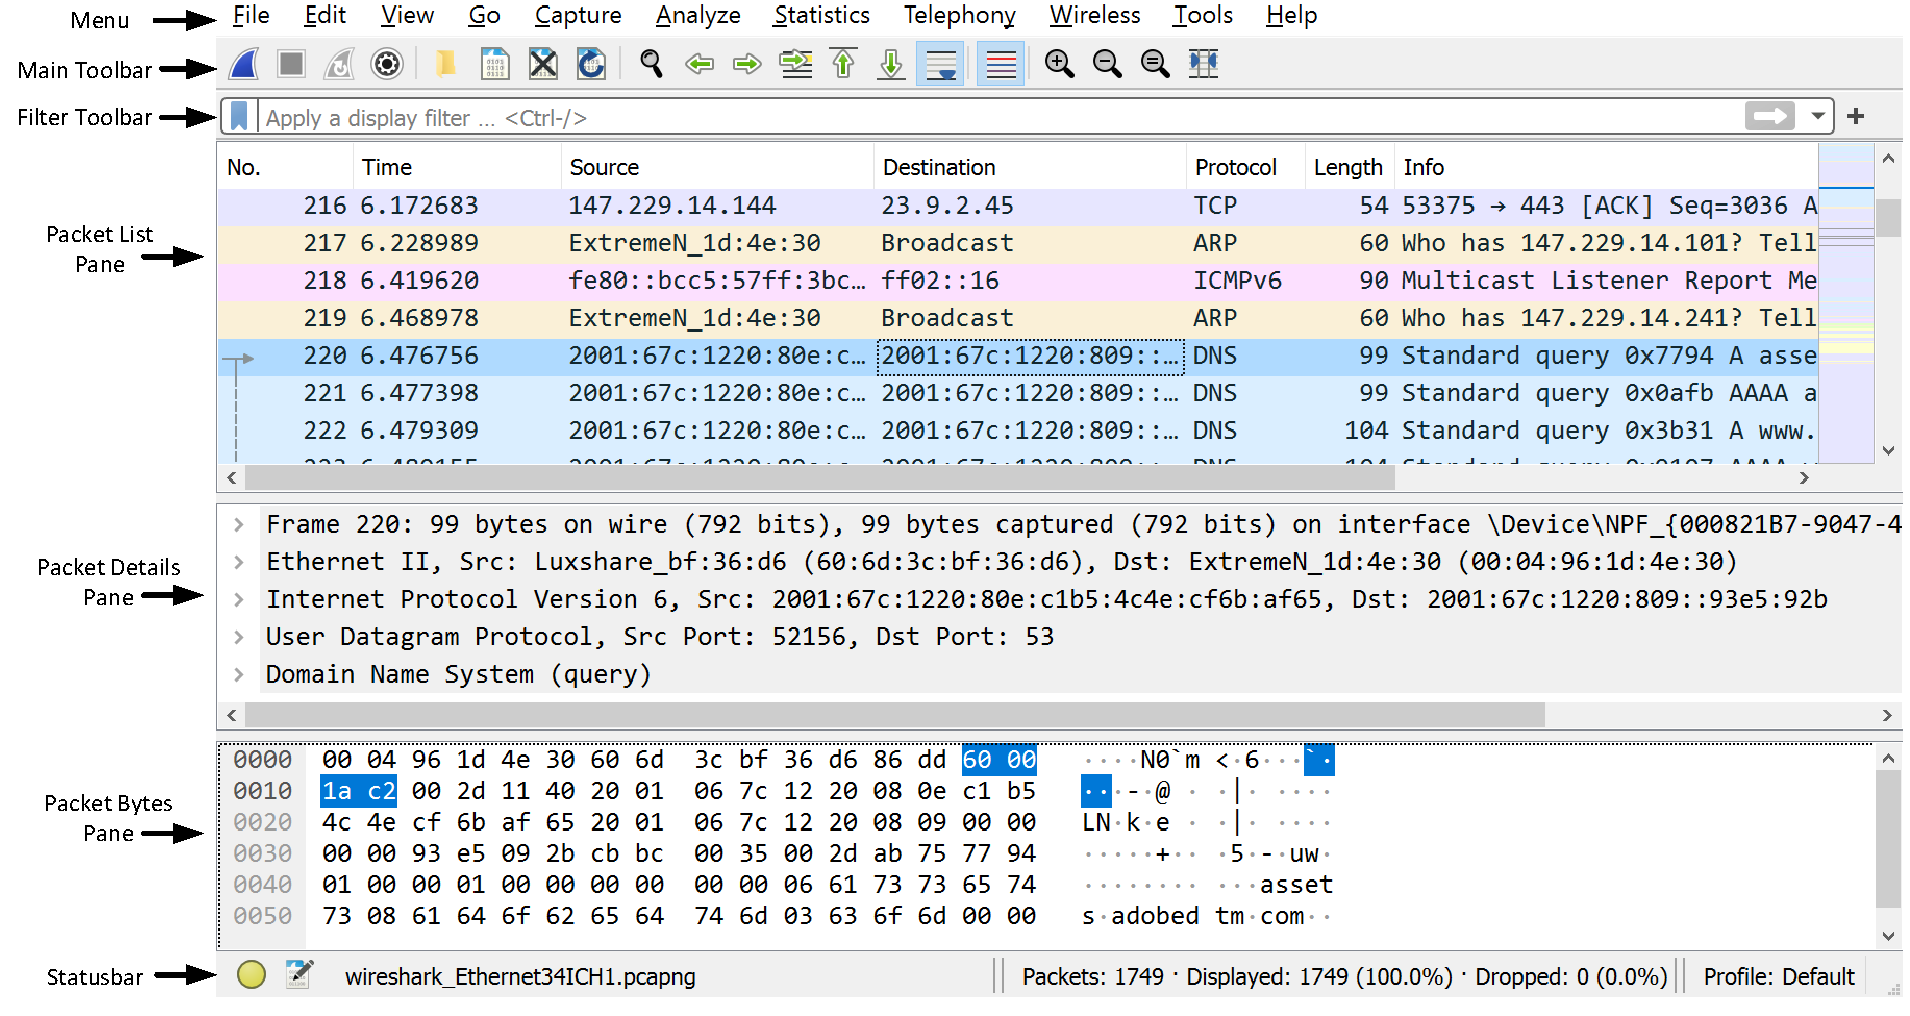
\includegraphics[width=170mm]{fig/wireshark-layout.pdf}
  \caption{Wireshark}\label{fig:wireshark-layout}
\end{figure}

\subsection{Zachytávání provozu (Packet Capturing)}
Následující kroky popisují proces zachytávání paketů v programu Wireshark:
\begin{enumerate}
  \item Zachytávat provoz můžeme z vybraného síťového rozhraní nebo z~více rozhraní najednou. Rozhraní vybereme v menu \texttt{Capture -> Options}.
  \item V nastavení Wiresharku je možné nastavit filtr pro výběr zachytávaných paketů (Capture Filter), pomocí kterého řekneme aplikaci, jaké pakety má zachytávat. Protože zpracování každého paketu je výpočetně náročné (dochází k parserování jednotlivých vrstev paketu a detekci protokolů), snížeme použití vstupního filtru výpočetní nároky na odchyt paketů. Políčko {\tt Capture Filter} umožňuje vybrat již předdefinovaný filtr nebo je zadat vlastní filtr, viz {\tt man pcap-filter}.
  \item Záchyt spustíme pomocí tlačítka \texttt{Start}.
  \item Odchycený provoz (tj. jednotlivé pakety spolu s časovými značkami) můžeme také uložit do souboru typu PCAP pro pozdější analýzu.
\end{enumerate}

\subsection{Výběr zachyceného provozu pomocí zobrazovacího filtru (Display Filter)}
Zachycené a zpracované pakety jsou zobrazeny v okně {\tt Packet List Pane}. Protože nás často zajímá pouze určitý provoz, např. komunikace HTTP s konkrétní stanicí, je vhodné využít zobrazovací filtr (Display Filter), který se nachází pod nástrojovou lištou. Pomocí tohoto filtru vybereme pouze pakety s požadovanou vlastností, např. filtr {\tt ip.addr == 147.229.8.12} vybere veškeré pakety, které mají danou zdrojovou či cílovou IP adresu. 

Základní operace pro vytváření zobrazovacího filteru je popsána v tabulce \ref{tab:display-filter}. 
\begin{center}
  \begin{table}[h]
    \centering
    \def\arraystretch{1.2}
    \begin{tabular}{|l|l|}
      \hline
      \textbf{Porovnávání} & \texttt{==, >=, <=, !=, contains}\\
      \textbf{Logické operátory} & \texttt{||, or, \&\&, and, !, not}\\
      \textbf{Kombinace filtrů} & \texttt{(ip.src==192.168.0.105 and udp.port==53)}\\
      \textbf{Filtrování na základě existence pole} & \texttt{http.cookie or http.set\_cookie}\\
      \textbf{Filtrování specifických bytů} & \texttt{eth.src[4:2]==22:1b}\\
      \textbf{Regex filtrování} & \texttt{http.host \&\& !http.host matches ".com"}\\
      \hline
    \end{tabular}
    \caption{Syntax zobrazovacího filtru (Display Filter)}\label{tab:display-filter}
  \end{table}
\end{center}

\subsection{Zobrazení toků (Flow Graph)}
Wireshark umožňuje zobrazit časovou posloupnost komunikace pomocí tzv. grafu toků zvaného \texttt{flow graph}, viz menu \texttt{Statistics -> Flow Graph}. Graf toků zobrazuje komunikaci mezi jednotlivými zařízeními definovanými IP adresou, viz obrázek \ref{fig:flow-graph}. Pomocí grafu toků můžeme vidět, jak často spolu stanice komunikují, jaké zprávy a v jakém pořadí si posílají a další.

\begin{figure}[h]
  \centering
  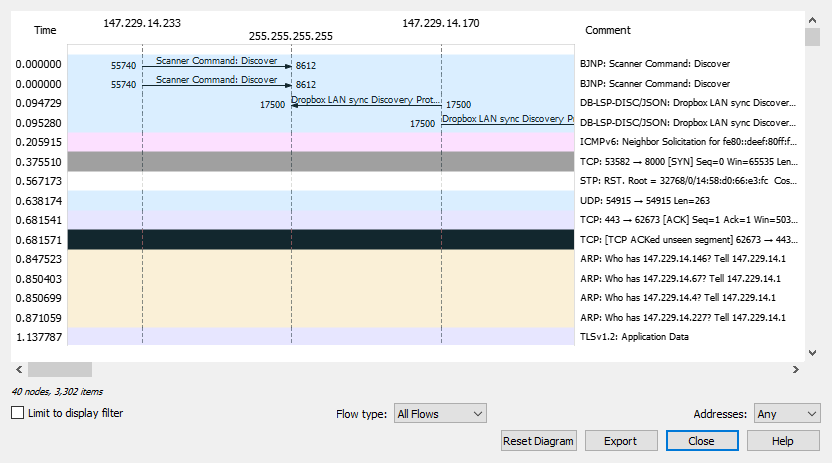
\includegraphics[width=110mm]{fig/flow-graph.png}
  \caption{Flow Graph}\label{fig:flow-graph}
\end{figure}

\subsection{Zobrazení obsahu toku (Stream Analysis)}
Wireshark zachytává jednotlivé pakety. Pokud chceme sledovat průběh celé komunikace včetně obsahu, můžeme  zobrazit danou komunikaci (streamu) pomocí volby \texttt{Flow <protokol> Stream}, např. TCP či UDP spojení, HTTP spojení apod. Zobrazení toku provedeme tak, že vybereme jeden zachycený paket daného toku, klikneme na něj pravým tlačítkem myši a vybereme volbu  \texttt{Follow <protokol> Stream}. Příklad obsahu HTTP komunikace je na obrázku \ref{fig:follow_stream}.

\begin{figure}[h]
  \centering
  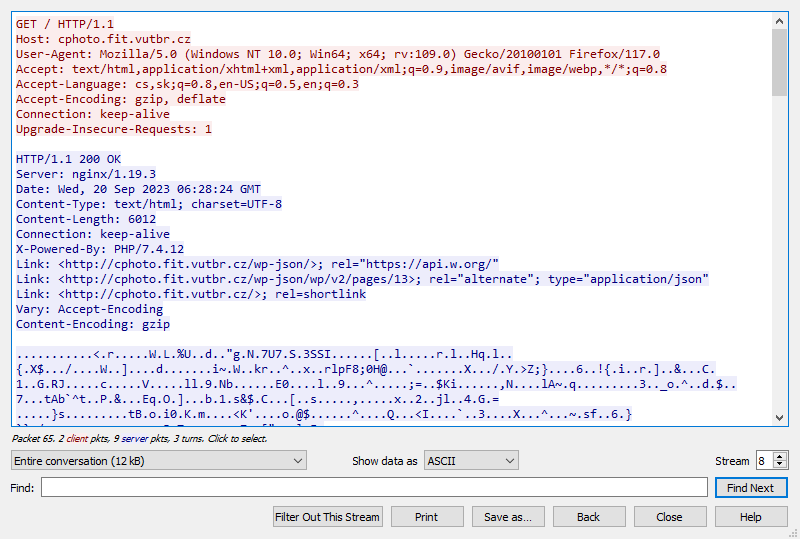
\includegraphics[width=110mm]{fig/follow_stream.png}
  \caption{Zobrazení toku HTTP}\label{fig:follow_stream}
\end{figure}

\subsection{Časové značky}
Každý paket obsahuje časovou značku svého záchytu. Zobrazení časové značky závisí na nastavení Wiresharku. Wireshark umožňuje zobrazit čas jako časovou značku obsahující datum a čas záchytu, absolutní čas, relativní čas od začátku záchytu komunikace a další. Formát času můžeme nastavit v menu \texttt{View -> Time Display Format}, viz obrázek \ref{fig:time-stamps}. Pro některé účely je vhodnější vidět pouze relativní čas od začátku záchytu paketů, pro jiné je potřeba znát absolutní čas záchytu. 

\begin{figure}[h]
  \centering
  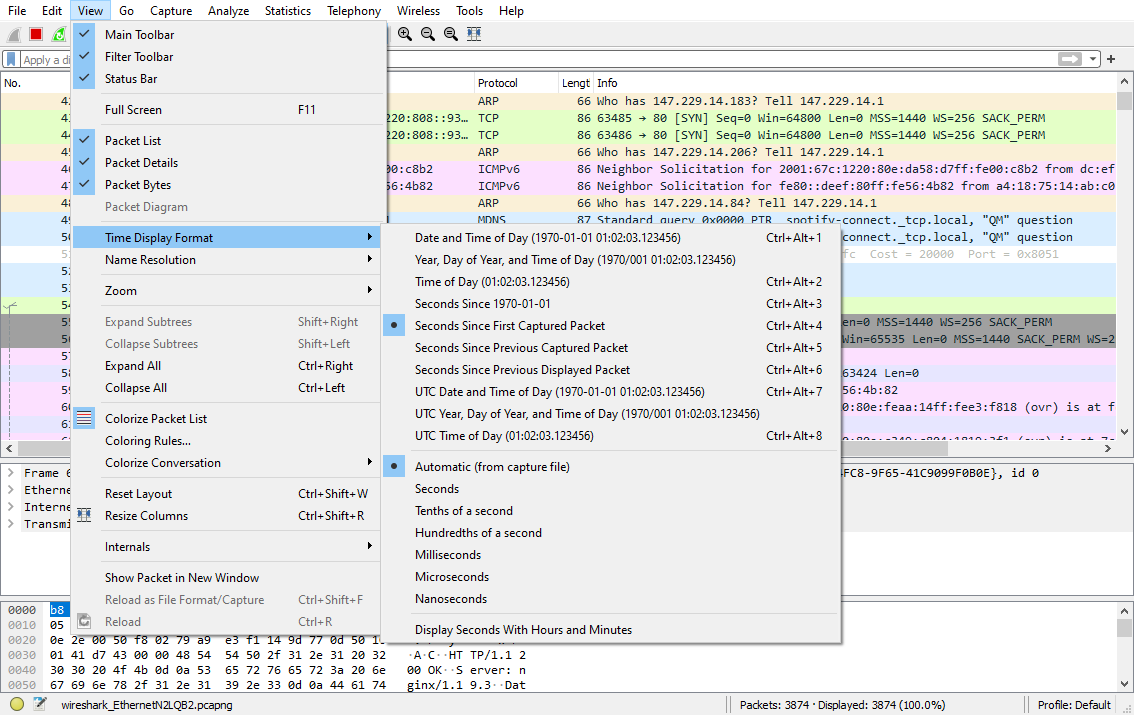
\includegraphics[width=110mm]{fig/time-stamps.png}
  \caption{Nastavení formátu časových značek}\label{fig:time-stamps}
\end{figure}


\clearpage
\section{Konfigurace síťování koncových zařízení}
\label{ipconfig}

\subsection{Manuální konfigurace IP adres}\label{ip_manual}
Pro manuální konfiguraci IP adres v operačním systému Linux je možné využít příkaz {\tt ip}:
\begin{itemize}
  \item \verb_ip link_, \verb_ip addr_ -- zobrazí aktuální konfiguraci síťových rozhraní
  \item \verb_ip link set <rozhraní> up/down_ -- zapne/vypne síťového rozhraní
  \item \verb_ip addr add/del <IP adresa>/<prefix> dev <rozhraní>_ -- přidá/odstraní IP adresy 
  \item \verb_ip addr flush dev [rozhraní]_ -- odstraní všechny IP adresy z daného rozhraní
  \item \verb_ip route_ -- zobrazí směrovací tabulku na počítači
  \item \verb_ip route add default via [IP adresa]_ -- nastaví výchozí bránu (default gateway)
\end{itemize}

Manuální nastavení IP adres pomocí příkazu {\tt ip} platí do nejbližšího restartu systému. Pro trvalé nastavení IP adres je potřeba použít grafické rozhraní {\tt Network Manager}, které je dostupné přes menu \textit{Settings/Network}.

\subsection{Dynamická konfigurace IPv4 pomocí DHCP}\label{dhcp}
Pro dynamickou konfiguraci IP adres je potřeba, aby byl na síti dostupný server DHCP. Pomocí protokolu DHCP provádí nejen konfiguraci IP adres, ale  nabízí klientům DHCP řadu dalších parametrů, které jsou potřeba ke konfiguraci daného zařízení, například adresy serverů DNS, WINS apod. 

Na cvičeních budeme používat implementace DHCP serveru a klienta zvanou ICS DHCP (Internet Systems Consortium DHCP). Pro konfiguraci DHCP serveru se používá konfigurační soubor \verb_/etc/dhcp/dhcpd.conf_ a systémová služba \texttt{isc-dhcp-server.service}.

Příklad nastavení rozsahu přidělovaných adres v konfiguračním souboru serveru DHCP:
\begin{verbatim}
Formát:
 option domain-name-servers < seznam IP adres DNS serverů>;
 subnet <IP adresa sítě> netmask <maska> {
    range <první IP adresa rozsahu> <poslední IP adresa rozsahu>;
 }
Příklad:
  option domain-name-servers ns1.isc.org, ns2.isc.org; # lokální DNS servery
  subnet 204.254.239.0 netmask 255.255.255.224 {       # podsíť 
      option routers 204.254.239.1;                    # výchozí brána
      option domain-name "test.isc.org";               # implicitní doména DNS 
      default-lease-time 120;                          # doba platnosti IP adresy
      range 204.254.239.10 204.254.239.30;             # rozsah přidělovaných IP adres
  }
\end{verbatim}
Podrobnější informace o~konfiguračních parametrech serveru DHCP lze najít v~manuálových stránkách {\tt man dhcpd.conf}, případně {\tt man dhcpd}.

Jako klienta DHCP budeme používat aplikaci \texttt{dhclient}. Úkolem klienta DHCP je požádat protokolem DHCP o konfigurační parametry dané stanice (přesněji řečeno síťového rozhraní). Klient může být spuštěn pro konkrétní síťové rozhraní nebo na všech rozhraních. Přes rozhraní, na kterém je klient spuštěn, posílá dotazy serveru DHCP. Pokud nevíme, na kterém rozhraní server DHCP pracuje, je vhodné pustit klienta bez parametrů, kdy pošle dotaz s žádostí o konfiguraci na všechna aktivní síťová rozhraní. 
\begin{verbatim}
dhclient -v [rozhraní]
\end{verbatim}
Argument \texttt{-v} vypíše detailní informace o průběhu konfigurace.
%Chybu týkající se {\tt smbd.service} někdy zobrazovanou v~laboratoři můžete ignorovat.

\subsection{Dynamická konfigurace IPv6}\label{dynipv6}
Dynamická konfiguace IPv6 probíhá zcela jiným způsobem, než konfigurace DHCP u sítí s protokolem IPv4. Dynamický konfigurace IPv6 probíhá třemi různými způsoby:
\begin{itemize}
  \item {\bf Autokonfigurace (SLAAC, Stateless Autoconfiguration)} \cite{rfc4862} -- autokonfigurace slouží ke konfiguraci síťových rozhraní IPv6 bez použití serveru DHCPv6. Při autokonfiguraci si připojený klient sám vytvoří adresu IPv6 z prefixu sítě (prvních 64 bitů) a identifikátoru rozhraní (spodních 64 bitů). Prefix sítě získá stanice zasláním zprávy ICMPv6 RS (Router Solicitation) na multicastovou adresu všech směrovačů v síti. Směrovač odpoví zprávou ICMPv6 RA (Router Advertisement), která obsahuje prefix sítě, L2 adresu směrovače, případně další parametry. Z adresy IPv6 odesilatele získa klientská stanice adresu výchozí brány, z odpovědi RA prefix sítě a adresu rozhraní (spodních 64 bitů adresy IPv6) si vygeneruje ze své MAC adresy mechanismem EUI-64 (rozšíření MAC adresy na 64 bitů) či si vygeneruje 64 bitů náhodně.
  \item {\bf Bezstavový server DHCPv6 (Stateless DHCPv6)} \cite{rfc8415} -- v tomto případě získá klientská stanice prefix sítě a výchozí bránu ze zprávy Router Advertisement jako u autokonfigurace. Bezstavový server DHCPv6 v tomto případě neslouží k přidělení IP adresy, ale k zaslání dalších konfiguračních parametrů, např. seznamu serverů DNS, domény DNS a další. Klientská stanice tedy pošle na server DHCPv6 (s využitím multicastové adresy) dotaz typu {\tt Information-request}, ve kterém uvede požadované parametry pro konfiguraci. Pokud je v síti nainstalován bezstavový server DHCPv6, zprávou {\tt Reply} pošle požadované nastavení.
  \item {\bf Stavový server DHCPv6 (Stateful DHCPv6)} \cite{rfc8415} -- klient posílá žádost {\tt Solicit} pro vyhledání serveru DHCPv6. Jakýkoliv server DHCPv6 odpoví zprávou {\tt Advertise}, ve které uvede nabízenou adresu IPv6, dobu platnosti a ostatní konfigurační parametry (servery DNS, doménu DNS). Klient odpoví žádostí {\tt Request}, ve které uvede identifikátor serveru, se kterým komunikuje, a konfigurační parametry, které požaduje. Server potvrdí přidělení parametrů zprávou {\tt Reply}. 
\end{itemize}

Na počítačích v~laboratoři lze využít službu {\tt radvd.service}, která vysílá zprávy Router Advertisement (RA). Aplikaci je možno nakonfigurovat v souboru {\tt /etc/radvd.conf}.

Příklad konfigurace:
\begin{verbatim}
interface <rozhraní>
{
    AdvSendAdvert on;
    MaxRtrAdvInterval <Max počet sekund mezi zprávami RA, min 4>;
    prefix <prefix>/<délka prefixu>
    {
        AdvOnLink on;
        AdvAutonomous on;
        AdvRouterAddr on;
    };
};
\end{verbatim}
Přehled všech možností konfigurace poskytnou manualové stránky {\tt man radvd} a {\tt man radvd.conf}.

Pro zasílání zpráv RA je potřeba povolit směrování IPv6 provozu:
\begin{verbatim}
sysctl net.ipv6.conf.all.forwarding=1
\end{verbatim}

Součásti balíčku radvd je i aplikace {\tt radvdump}, která slouží k analýze zpráva RA: naslouchá na síťových rozhraních a zobrazuje zachycené zprávy na standardní výstup.

\newpage
%%%%%%%%%%%%%%%%%%%%%%%%%%%%%%%%%%%%%%
\section{Synchronizace času protokolem NTP (Network Time Protocol)}\label{ntp}
Protokol NTP \cite{rfc1305} umožňuje synchronizovat čas mezi uzly v~síti. Jeho úkolem je přenášet časové informace z primárních časových serverů s přesnými hodinami na ostatní servery a klienty. Protokol NTP při synchronizaci bere v úvahu proměnlivou dobou přenosu paketu, zpoždění paketu a další parametry. NTP organizuje servery hierarchicky do úrovní: primární servery NTP předávají časové informace sekundárním serverům, ty je pak předávají serverům nižší úrovně atd. Úroveň vzdálenosti od přesného zdroje času se vyjadřuje veličinou {\em stratum}. Nejnižší hodnota 0 označuje referenční zdroj přesného času (např. GPS). Stratum 1 označuje primární servery, které jsou synchronizovány právě s~referenčním zdrojem. Stratum 2 jsou servery synchronizovány se servery stratum 1 atd. \cite{rfc5905}.

Implementaci protokolu NTP zajišťuje balík aplikací {\em ntp}. Tento balík se skládá z~několika
aplikací. V~rámci laboratorního cvičení budeme používat aplikace {\tt ntpd} či {\tt ntpq} (viz část \ref{sec:ntpq}). Chrony\footnote{Viz \url{https://chrony.tuxfamily.org/}.} nabízí alternativní
implementaci NTP.

\subsection{Aplikace {\tt ntpd}}
Aplikace {\tt ntpd} (NTP démon) slouží k synchronizaci času pomocí NTP. Může pracovat v režimu klienta i serveru. Aplikace běží na pozadí a neustále synchronizuje čas s~nastavenými servery, případně upravuje lokální čas. Úprava lokálního času se provádí úpravou rychlosti běhu lokálního času. Pokud je lokální čas pozadu, resp. se předbíhá, tak se systémové hodiny {\em zrychlují}, resp. {\em zpomalují}. Tento způsob úpravy času znamená, že pokud je čas odchýlen o~několik minut, bude nějakou dobu trvat, než dojde k synchronizaci. Na druhou stranu se tak zabrání skokové změně a navíc čas se nikdy neposune do minulosti. Pokud je lokální čas odchýlen o~více než 1000 sekund (necelých 17 minut), aplikace to vyhodnotí jako chybu a skončí. Pokud se tak stane, objeví se zpráva v~systémovém logu.

Zda aplikace běží, lze zjistit například příkazem {\tt ntpq -p}. Pokud není démon {\tt ntpd} spuštěn, skončí aplikace hláškou {\em ntpq: read: Connection refused}. 

Službu NTP je možné spustit příkazem:
\begin{verbatim}
systemctl start ntp.service
\end{verbatim}
Aby se předešlo problému v~případě, kdy např. hardwarové hodiny jdou špatně a při vypnutí může dojít k~odchýlení lokálního času o~více než 17 minut, je možné vynutit okamžité nastavení času příkazem
\begin{verbatim}
ntpd -qg  # -g vypne kontrolu odchylky a nastaví čas bez ohledu na velikost odchylky
          # -q ukončí běh démona poté, co byl čas nastaven
\end{verbatim}

\subsubsection{Konfigurace}
Základním konfiguračním souborem je {\tt /etc/ntp.conf}. Tento konfigurační soubor obsahuje mnoho
konfiguračních voleb. Nastavení serverů NTP zajišťuje volba {\tt server}, za níž následuje adresa nebo jméno NTP serveru. Tato volba se může vyskytovat v konfiguračním souboru opakovaně. Pomocí této volby se aplikace {\tt ntpd} přepne do role klienta, který může využít k sychronizaci svého času více serverů NTP. V režimu klient se lokální hodiny synchronizují podle času ze vzdáleného serveru NTP. 

Kromě režimu klient může {\tt ntpd} pracovat v režimu {\em peer}, která umožňuje, aby se vzdálený server synchronizoval podle lokálních hodin. To je užitečné v případě, že je v síti více serverů NTP, které mohou mít lepší zdroj času. Zároveň to řeší problém výpadků serverů. 

V konfiguraci můžeme také zvolit možnosti komunikace typu {\em broadcast} nebo {\em manycastclient}, za nimiž následuje broadcastová či multicastová adresa. Na tyto adresy server NTP posílá periodické zprávy s aktuálním stavem hodin. Pro multicastové přenosy se využívají skupiny definované IANA pro protokol NTP, tj. 224.0.1.1 pro IPv4 a ff05::101 pro IPv6. 

Jinou užitečnou volbou je {\em restrict}, která slouží pro řízení přístupu. Aplikací {\tt ntpd} mohou být zaslány různé požadavky přes síť (například pomocí {\tt ntpq}). Je vhodné povolit některé dotazy jen z~určitého uzlu nebo podsítě. Využití této volby může být také užitečné v~případě, že se pro nastavování času využívá broadcastu nebo multicastu a není žádoucí, aby takto vyslanou informaci klienti akceptovali z~libovolného zdroje. Základní tvar tohoto příkazu je:
\begin{verbatim}
restrict <adresa> [mask <maska>] [<jeden či více příznaků>]
\end{verbatim}

Příznak definuje omezení pro danou adresu/síť:
\begin{itemize}
  \item ignore -- zahazovat všechny pakety
  \item nomodify -- povolí pouze dotazy, požadavky měnící stav serveru jsou zahazovány
  \item noquery -- zakáže dotazy pomocí {\tt ntpq}, synchronizace času není ovlivněna
  \item notrust -- zahazovat neautentizované pakety
\end{itemize}
Další příznaky a jejich popis lze nalézt v~manuálových stránkách {\tt man ntp.conf}.

%%Pokud budou aplikace {\tt ntpq} a {\tt ntpdc} (viz podkapitola \ref{sec:ntpq} používané i pro změnu konfigurace, pak je nezbytné nastavit autentizaci. Protokol nabízí možnost využití symetrické i asymetrické kryptografie. Pro použití symetrické kryptografie jsou k~dispozici tyto volby:
%%\begin{itemize}
%%  \item keys -- tato volba má jeden parametr, který udává název souboru, který obsahuje používané klíče (obvykle {\tt /etc/ntp.keys},
%%  \item trustedkey -- výčet klíčů, kterým se bude důvěřovat,
%%  \item requestkey -- seznam klíčů, které mohou být použity aplikací {\tt ntpdc},
%%  \item controlkey -- seznam klíčů, které mohou být použity aplikací {\tt ntpq}.
%%\end{itemize}
%%Formát souboru {\tt /etc/ntp.keys} má následující tvar:
%%\begin{verbatim}
%%<číslo klíče> <typ> <heslo>
%%\end{verbatim}
%%Typ může nabývat čtyř hodnot. Hodnoty {\tt S} a {\tt N} používají bitový formát a běžně se neužívají. Hodnoty {\tt A} a {\tt M} používají textový řetězce délky 1 až 8 znaků a určují způsob zašifrování při přenosu. Nejčastěji se užívá možnost {\tt M}, která značí použití DES nebo MD5. Příklad souboru pak může vypadat následovně:
%%\begin{verbatim}
%%1 M heslo1
%%2 M secret
%%3 M passwd
%%\end{verbatim}
%%Konfigurace v~{\tt /etc/ntp.conf} potom vypadá:
%%\begin{verbatim}
%%keys /etc/ntp.keys
%%trustedkey 1 2 3
%%requestkey 2
%%controlkey 1 3
%%\end{verbatim}
%%
%%Toto značí, že důvěryhodné jsou všechny tři klíče. Aplikace {\tt ntpdc} se může autentizovat pouzde klíčem 3 a aplikace {\tt ntpq} klíči 1 a 3.   
%%
  
\subsection{Aplikace {\tt ntpq}}\label{sec:ntpq}
%% Tyto dvě aplikace nabízejí v~podstatě podobné možnosti konfigurace serveru NTP. Rozdílů je mezi těmito programy několik. První, který byl již uveden výše, je v~tom, že každá z~těchto aplikací může používat jinou množinu klíčů. Podstatnější rozdíl z~uživatelského hlediska je v~tom, že aplikace {\tt ntpdc} má přesně definovaný výčet příkazů, které lze aplikovat, a proto může měnit jen to, co je v~aplikaci definováno. Naproti tomu {\tt ntpq} disponuje příkazem {\tt :config}, kterému se jako parametry předávají konfigurační volby, které se používají v~souboru {\tt /etc/ntp.conf}. Další rozdíl je ve formátu zpráv, pomocí kterých komunikují se serverem.

Aplikace {\tt ntpq} (NTP query) se používá pro zasílání dotazů serveru NTP {\tt ntpd} z důvodu sledování běhu a výkonnosti, případně zjišťování aktuálního stavu. {\tt ntpq} zasílá zprávy přes síťové rozhraní, i když běží lokálně či vzdáleně. Tato aplikace může měnit konfiguraci {\tt ntpd} za běhu. Možnost změny parametru přes síť může být nežádoucí, proto je vhodné omezit pomocí volby {\em restrict} přístup pouze přes rozhraní {\tt loopback}. 

Příklad výstupu volání {\tt ntpq -p}:

\begin{verbatim}
     remote           refid      st t when poll reach   delay   offset  jitter
==============================================================================
+rhino.cis.vutbr 248.205.243.78   3 u  425 1024  377   10.070   -4.280  10.575
+tik.cesnet.cz   195.113.144.238  2 u  622 1024  377    4.796   -3.464  16.528
*tak.cesnet.cz   .GPS.            1 u  364 1024  377    5.008   -3.625   6.228
\end{verbatim}

Výpis obsahuje následující hodnoty:

\begin{description}

  \item[remote] Klient se synchronizuje vůči třem serverům: rhino.cis.vutbr.cz,
    tik.cesnet.cz a tak.cesnet.cz. Hvězdičkou je označený primární zdroj času,
    plusem sekundární zdroje času.

  \item[refid] Primární zdroj času pro vzdálený server NTP.

  \item[stratum] Počet skoků od vzdáleného serveru k přesnému zdroji času (1
    znamená, že zdroj přesného času je přímo připojen, 16 znamená, že vzdálený
    server je nedosažitelný).

  \item[when] Počet sekund od posledního kontaktu se serverem.

  \item[poll] Počet sekund mezi jednotlivými dotazy protokolem NTP.

  \item[reachability] Úspěšnost posledním 8 pokusů o kontakt vzdáleného serveru
    v osmičkové soustavě. (1 znamená pouze poslední pokus uspěl, 377 znamená
    všech 8 posledních pokusů uspělo).

  \item[delay, offset, jitter] Zpoždění, posun a jitter -- charakteristiky
    vzdáleného zdroje času, podle kterého se volí primární a sekundární zdroje
    času.
\end{description}

\newpage
%%%%%%%%%%%%%%%%%%%%
\section{Secure Shell}
\label{ssh}

Základní funkcí protokolu Secure Shell (SSH) \cite{rfc4253} je umožnění bezpečného přístupu
 ke vzdálenému počítači přes nezabezpečenou síť. Díky tomu, že je protokol SSH navržen obecně,
 lze pomocí něj zabezpečovat i další služby, jako je např. X Window, přístup ke vzdálenému
 souborovému systému (SFTP, sshfs, scp), tunelování portů TCP apod. Protokol SSH zajišťuje
 šifrování dat, autentizaci, integritu dat a volitelně také kompresi přenášených dat.

V~rámci předmětu ISA se zaměříme pouze na malou část možností, které protokol SSH přináší. V~rámci
 cvičení si vyzkoušíme protokol SSH pro terminálový přístup ke vzdálenému stroji a ukážeme si
 využití přihlašování ke vzdálenému počítači pomocí klíčů. Dále si vyzkoušíme, jak využít SSH
 k~vytvoření jednoduché HTTP proxy.

Jednou z~nejčastěji používaných aplikací pro využití protokolu SSH je sada programů OpenSSH.
 Balíček programů obsahuje kromě klienta {\tt ssh} i serverovou aplikaci {\tt sshd}, program
 pro generování SSH klíčů {\tt ssh-keygen}, agenta pro usnadnění práce s~SSH klíči {\tt ssh-agent}
 a další. My budeme předpokládat, že na počítačích, na které se budeme snažit připojit
 již běží SSH server {\tt sshd}. Konfigurace tohoto programu je nad rámec tohoto manuálu. Zájemci
 mohou nalézt podrobnější informace v~manuálové stránce {\tt sshd\_config(5)}, či v~jiných návodech.

\subsection{Připojení ke~vzdálenému počítači}

Pro připojení se k~počítači pojmenovaném \emph{h01} a otevření příkazového řádku na vzdáleném
 stroji je možné použít příkaz:

\begin{verbatim}
ssh h01
\end{verbatim}

Příkaz ssh má celou řadu parametrů, které jsou detailně popsány v~manuálové stránce {\tt ssh(1)}.
 Z~těch nejčastěji používaných zmíníme alespoň změnu uživatelského jména ({\tt -l}), specifikování
 TCP portu vzdáleného serveru ({\tt -p}), zvýšení výřečnosti programu ({\tt -v}, tento parametr
 lze použít i vícekrát), zapnutí tunelování protokolu X Windows ({\tt -X}, {\tt -Y})
 a přesměrování portů ({\tt -L}). Často zadávané parametry se specifikují v konfiguračním souboru
 \verb|~/.ssh/config|. Popis tohoto souboru obsahuje manuálová stránka {\tt ssh\_config(5)}.

Po připojení ke vzdálenému serveru jsou informace o~použitém spojení dostupné např. v~rámci
 proměnných prostředí. Proměnné prostředí související s~protokolem SSH je možné zobrazit
 příkazem {\tt env | grep SSH}. Následující výpis ukazuje příklad proměnných po připojí
 k~serveru {\tt merlin} protokolem IPv6:

\begin{verbatim}
local $ ssh merlin6.fit.vutbr.cz 
merlin $ env | grep SSH
SSH_CLIENT=2001:67c:1220:80c:e138:4d11:c04c:c675 54514 22
SSH_TTY=/dev/pts/30
SSH_CONNECTION=2001:67c:1220:80c:e138:4d11:c04c:c675 \
  54514 2001:67c:1220:8b0::93e5:b013 22
\end{verbatim}

Z~výpisu vidíme, že připojení bylo realizováno na IPv6 adresu {\tt 2001:67c:1220:8b0::93e5:b013}
 z~počítače s~adresou {\tt 2001:67c:1220:80c:e138:4d11:c04c:c675}. Byl použit zdrojový port č. 54514,
 na straně serveru byl použit standardní protokol 22. Po připojení využíval vzdálený uživatel
 terminál č. 30. Odhlášení ze vzdáleného počítače probíhá standardními prostředky pro ukončení
 shellu, např. příkaz {\tt exit}, nebo vložení konce souboru klávesovou zkratkou {\tt Ctrl-D}.

\subsection{Kopírování souborů mezi počítači}

Pro kopírování souborů protokolem SSH je často využívaná utilita {\tt scp}. Cesta na vzdáleném
 serveru je specifikována v~následujícím formátu: {\tt uživatel@jménoserveru:cesta}.
 Následující příkaz zkopíruje lokální soubor isa na vzdálený počítač h01 do
 složky fit umístěné v~domovské složce uživatele student.

\begin{verbatim}
scp isa student@h01:fit/
\end{verbatim}

\subsection{SSH jako proxy a tunelování portů}
Díky velmi obecné implementaci lze protokolem SSH tunelovat jakýkoli typ provozu. Je tedy možné
 např. zajistit šifrování provozu po určitou část komunikace, konkretně po stanici, ke které
 se připojujeme SSH protokolem, nebo přesměrovat provoz z~některého portu na jiný port. Následujcí
 příkaz nám otevře SSH spojení, které pak můžeme použít jako proxy ve webovém prohlížeči.

\begin{verbatim}
  ssh -D 12345 -N student@sshserver
\end{verbatim}

Po autentizaci stačí pak v~prohlížeči zadat jako nastavení proxy server localhost s~portem 12345
 a~provoz bude směrován nejprve na localhost, poté půjde ssh spojením na sshserver, kde bude převeden
 na běžný HTTP/HTTPS provoz a~poslán dále. 

\subsection{Klíče protokolu SSH}

Klíče protokolu SSH mají několik výhod. Díky nim není nutné posílat heslo pro přístup ke vzdálenému
 stroji přes síť, byť v~šifrované podobě. Délka používaných klíčů znesnadňuje potenciálnímu
 útočníkovi útok hrubou silou, protože síla klíče bývá typicky vyšší než síla běžně používaných
 hesel. Ve spojení s~agentem pro správu klíče může uživatel přistupovat ke vzdálenému serveru bez
 nutnosti opakovaného zadávání hesla. Agent může být nastaven, aby pro použitý klíč nevyžadoval
 heslo po zbytek sezení, či po určitý počet minut.

SSH klíč se obvykle generují utilitou {\tt ssh-keygen}. Po spuštění bez parametrů je vytvořen pár
 klíčů algoritmem RSA o~délce 2048\,B. Uživateli je nabídnuto umístění souboru,
 které může změnit. Dále je uživatel požádán o~zadání passfráze, od které se očekává, že bude
 silnější než heslo. Parametr {\tt -t} nastavuje jiný typ šifrovacího algoritmu,
 parametr {\tt -b} mění délku klíče, parametrem {\tt -f} specifikuje umístění souboru, parametr
 {\tt -C} upravuje popis klíče, další parametry popisuje manuálová stránka {\tt ssh-keygen(1)}.
 Následující příklad vygeneruje klíč o~délce 4096\,B, který nebude chráněn passfrázi:

\begin{verbatim}
ssh-keygen -t rsa -b 4096 -N "" -f ~/.ssh/nopass -C nopass
\end{verbatim}

Po vytvoření klíčů vzniknou dva soubory. Ten který je bez přípony {\tt .pub} je soukromý klíč,
 který by měl zůstat tajný a uživatel, který jej vytvořil by jej neměl dále distribuovat.
 Soubor s~příponou {\tt .pub} je určen pro volnou distribuci.

Podrobný popis použití klíčů během přihlašování najdete např. na \url{https://www.digitalocean.com/community/tutorials/understanding-the-ssh-encryption-and-connection-process}.

\subsection{Konfigurace použití klíčů}

Nejdříve je potřeba distribuovat soubor s~veřejným klíčem na vzdálený počítač. K~tomu slouží
 např. program {\tt scp}. Každý z~uživatelů si může specifikovat sadu klíčů pro přístup k~danému
 stroji v~souboru \verb|~/.ssh/authorized_keys|. Nový klíč do tohoto souboru přidáme např. takto
 (všimněte si, že se klíč přidává na konec souboru pomocí \verb|>>|):

\begin{verbatim}
cat id_rsa.pub >> ~/.ssh/authorized_keys
\end{verbatim}

Nyní se již můžeme připojit ke vzdálenému počítači pomocí vytvořených klíčů. Pokud jsme klíč
 na lokálním počítači umístili do výchozího umístění, je klíč použit automaticky. Pokud jsme
 zvolili jiné umístění, je potřeba program {\tt ssh} informovat o~umístění klíče parametrem
 {\tt -i}, nebo volbou {\tt IdentityFile} v~konfiguračním souboru. Informace o hledaných
 klíčích jsou zobrazeny po použití parametru {\tt -v}.


\newpage
%%%%%%%%%%%%%%%%%%%%
\section{Zabezpečení TLS (Transport Layer Security)}\label{tls}
Původní přenosové protokoly na počátky Internetu byly nešifrované. Požadavek na zabezpečení dat se objevil později v souvislosti se zveřejněním informací o masivním odposlechu internetových linek bezpečnostními službami na Wikileaks. S tím souvisí i následná snaha o ochranu dat a soukromí u veřejných služeb jako jsou DNS, Telnet, HTTP, SMTP, FTP, VoIP a další. Přestože standardy SSL (Secure Sockets Layer) vznikaly postupně od roku 1995  a standardy TLS od roku 1999 \cite{rfc2246}, jejich rozšíření spadá do let 2014-2018, kdy například šifrování webového provozu se z cca 50\% dostává na více jako 80\%\footnote{Viz \url{https://transparencyreport.google.com/https/overview?hl=en}}.

Protože velká část původních internetových protokolů šifrování nepodporovala (např. DNS, HTTP, SMTP, IMAP, FTP), začal se využívat koncept tunelování aplikačních protokolů přes protokoly SSL/TLS, která tak vytvářejí mezivrstvu mezi transportní a aplikační vrstvou, viz obrázek \ref{fig:tls}. Tato vrstva zajišťuje nejen šifrování, ale i autentizaci, integritu dat, bezpečnou výměnu klíčů a další funkce. Výhodou tohoto přístupu je, že přidání podpory SSL/TLS je pro existující aplikace transparentní, tzn. není nutné provádět jakoukoliv změnu stávajících protokolů.

\begin{figure}[h]
  \centering
%    
\includegraphics[width=0.3\textwidth]{fig/vrstvy-ssl}
    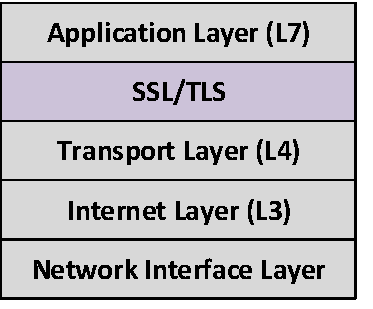
\includegraphics[width=0.3\textwidth]{fig/tls.pdf}
  \caption{Rozšíření modelu TCP/IP o vrstvu SSL/TLS.}
 \label{fig:tls}
\end{figure}

Původní proprietární protokol SSL (navržený firmou Netscape Corporation) byl postupně nahrazen protokolem TLS \cite{RFC7568}. Aktuální doporučená verze protokolu TLS je 1.3~\cite{RFC8446}\footnote{Neformální popis popis standardu TLS je na \url{https://www.davidwong.fr/tls13/}.}.

TLS pracuje na principu klient -- server a vytváří obousměrný zabezpečený kanál pro komunikaci na aplikační vrstvě mezi klientem a serverem. TLS  zajišťuje následující typy zabezpečení:
\begin{itemize}
  \item {\em Autentizace} -- vždy ověřuje identitu serveru (tzv. jednostranná autentizace), která slouží k ochraně komunikace proti útokům typu MITM (Man In the Middle). Může implementovat i oboustrannou autentizaci, kdy klient poskytuje své autentizační údaje server. V praxi se tento přístup příliš nevyužívá. Pro ověřování identity se využívají veřejné klíče a certifikáty X.509, které jsou podepsány certifikační autoritou. 
  \item {\em Důvěrnost (utajení)} -- po navázání spojení a výměně konfiguračních parametrů je obsah přenášené komunikace šifrován. 
  \item {\em Integrita dat} -- TLS zajišťuje ochranu proti modifikaci, vložení či odebrání dat z přenášené komunikace pomocí tzv. kryptografického heše (např. MD4, SHA). 
\end{itemize}

Samotný protokol TLS se skládá ze dvou dílčích protokolů, které jsou součástí zprávy TLS:
\begin{itemize}
  \item \emph{Handshake protocol} se používá při navazování spojení a zajišťuje autentizaci komunikujících stran, výběr kryptografických algoritmů, výměnu parametrů a sdílených klíčů.
  \item \emph{Record protocol} zajišťuje bezpečný přenos mezi komunikujícími stranami.
\end{itemize}

\subsection{Certifikační autority}
Certifikační autorita (CA) je v asymetrické kryptografii subjekt, který vydává digitální (elektronické) certifikáty a ověřuje jejich pravost. Certifikát je elektronický dokument (popsaný v notaci X.500)  potvrzující příslušnost veřejného klíče k dané entitě (službě, serveru, osobě). Certifikační autorita na základě požadavku vygeneruje pro danou entitu dvojici veřejný a soukromý klíč a veřejný klíč s identifikací žadatele vloží do dokumentu zvaného certifikát. Struktura certifikátu je definována standardem X.509 a obsahuje následující informace \cite{rfc5280}:
\begin{itemize}
  \item jméno žadatele (subject)
  \item veřejný klíč žadatele (subject public key)
  \item informace o certifikátu (verze, sériové číslo, doba platnosti)
  \item informace o vydavateli (issuer)
  \item podpis certifikátu (certificate signature), algoritmus a parametry podpisu
\end{itemize}

Pro validaci certifikátu se využívá podpisu certifikační autority, která pomocí svého soukromého klíče podepíše vydaný certifikát. Ověření probíhá pomocí veřejného klíče CA. Jak můžeme ale veřejnému klíči CA důvěřovat? Tento klíč opět musí být podepsán, tzn. musí existovat certifikát, který ověřuje pravost veřejného klíče dané CA. Toto ověření provádí CA vyšší úrovně a vytváří se struktura důvěryhodnosti veřejných klíčů PKI (Public Key Infrastructure). 

Pro ověřování certifikátů nejvyšší úrovně se používají národní a nadnárodní certifikační autority, jejichž veřejné klíče jsou obvykle umístěny přímo ve webových prohlížečích a dalších programech, čímž usnadní uživatelům ověřování důvěryhodnosti webových certifikátů či jiných elektronicky podepsaných dokumentů. 

\subsection{Transparentnost certifikátů}
Aby bylo možné ověřit, že CA vydávají certifikáty poctivě, byl experimentálně zaveden mechanismus transparentnosti certifikátů. Zapojené CA veřejně ohlašují každý vystavený certifikát (případně pre-certifikát). Vydané certifikáty se shromažďují v logovacím souboru {\tt certificate transparency log}, kde může kdokoliv monitorovat nově
přidávané certifikáty a auditovat přítomnost certifikátu nalezených při prohlížení webu.

\newpage
%%%%%%%%%%%%%%%%%%%%%%%%%%%%%%%%%%%%%%
\section{Systém DNS (Domain Name System)}\label{dns}
Systém DNS slouží jako podpora internetové komunikace, kdy ukládá informace důležité ke správnému fungování počítačových sítí a služeb. Jednou z nejvíce využívaných služeb je překlad doménového jména na IP adresu a naopak, tzn. vyhledávání záznamů typu A, AAAA a PTR \cite{rfc1035,rfc3596}.

Mezi další důležité záznamy patří záznam {\tt MX}, který obsahuje adresu poštovního serveru pro danou doménu. Záznamy {\tt MX} jsou nezbytné pro správné fungování systému elektronické pošty nad SMTP. Pro vyhledávání serverů dalších služeb (např. SIP, XMPP a další) slouží záznamy typu {\tt SRV}, které lze v~současnosti využít pro služby SIP a XMPP \cite{rfc2782}.

Některé záznamy během vývoje internetu rozšířili svou funkci. Například záznamy typu {\tt TXT} byly původně používány pro uložení textových informací o dané doméně. V současné době se převážně využívají pro zajištění bezpečnosti softwarových služeb či přenosu elektronické pošty, kde záznam {\tt TXT} například obsahuje veřejný klíč pro službu DKIM (DomainKeys Identified Mail) \cite{rfc6376}).

Služba DNS pracuje na principu klient--server, kde klient (zvaný též resolver) posílá dotaz pro vyhledání informací v distribuované globálním systému DNS. Dotaz přijde na server DNS, který se snaží najít odpověď bud v lokální databázi (zónovém souboru) či paměti cache. Pokud odpověď nenajde lokálně, může se dotazovat dalších serverů (v případě rekurzivního dotazu). Proces vyhledání informací v systému DNS se nazývá {\em rezoluce}. 

\subsection{Konfigurace klienta DNS}
Co je klient DNS? Možná zvláštní otázka, nicméně definice klienta DNS není zcela jednoznačná. Za klientské programy lze považovat aplikace typu {\tt nslookup}, {\tt host} či {\tt dig}, což jsou programy, které komunikují se servery DNS. Všechny tyto programy pro svou činnost využívají soubor systémových rutin zvaný {\em resolver}, který je součástí operačního systému a implementuje zasílání dotazů na server DNS a zpracování odpovědí. Z uživatelského pohledu lze tedy za klienty DNS považovat aplikace typu {\tt nslookup}, z implementačního pohledu je klientem DNS {\em resolver}. Protože však aplikační programy typu {\tt nslookup} umožňují uživateli přistupovat k systému DNS, budeme je také nazývat klienty DNS.

Pro konfiguraci klienta DNS se využívají následující konfigurační soubory: {\tt /etc/hosts}, {\tt /etc/re\-solv.conf} a {\tt /etc/hosts.conf}. 
\begin{itemize}
  \item {\tt /etc/hosts} -- Tento soubor obsahuje statické mapování IP adres a doménových jmen. Vytváří se manuálně a využívá se například jako záloha v situaci, kdy není server DNS dostupný. Soubor {\tt /etc/hosts} obvykle obsahuje jen základní mapování lokální adresy {\tt localhost} na IP adresu. Do souboru můžeme vložit i další doménová jména a odpovídající IP adresy, viz následující ukázka. Formát souboru lze najít v manuálových stránkách {\tt man hosts}. 
\begin{verbatim}
::1         localhost localhost.my.domain
127.0.0.1   localhost localhost.my.domain
10.0.0.3    myfriend.my.domain myfriend
\end{verbatim}
  \item {\tt /etc/resolv.conf} -- Jedná se o konfigurační soubor resolveru DNS. Resolver DNS vytváří dynamické mapování (nejen) IP adres a doménových jmen zasíláním dotazů na server DNS. Konfigurační soubor obsahuje například název implicitní domény (parametr {\tt search}). Ta se doplňuje za doménová jména, která nejsou plně kvalifikovaná, např. doménové jméno {\tt merlin} se při dotazování DNS automaticky rozšíří o implicitní doménu na {\tt merlin.fit.vutbr.cz}. Dále obsahuje konfigurační soubor {\tt /etc/resolv.conf} seznam serverů DNS (parametr {\tt nameserver}), na které lokální počítač posílá dotazy DNS. Popis všech dostupných parametrů lze najít na manuálových stránkách {\tt man resolv.conf}. Konfigurace souboru je buď manuální, tj. administrátor ručně vloží IP adresy lokálních serverů DNS, implicitní doménu apod. do tohoto souboru, nebo se konfigurace vytvoří z DHCP. Pokud je nastavena možnost konfigurace DHCP, pak se manuálně vložené data přepíšou hodnotami z DHCP. Příklad konfigurace lokálního klienta DNS na FIT:
\begin{verbatim}
# Generated by resolvconf
search fit.vutbr.cz             # implicitní doména
nameserver 147.229.9.43         # seznam serverů DNS
nameserver 147.229.8.43
\end{verbatim}
  \item {\tt /etc/host.conf} -- U rezoluce doménových jmen je potřeba stanovit, zda má přednost statický překlad uložený v souboru {\tt /etc/hosts} nebo dynamické vyhledávání systému DNS přes {\tt resolver}. Pořadí rezoluce definuje konfigurační soubor {\tt /etc/host.conf}, který je automaticky generován z konfiguračního souboru {\tt nsswitch.conf}, viz {\tt man nsswitch.conf}. Soubor {\tt /etc/host .conf} udává pořadí zdrojů překladu DNS. Standardně se nejprve využívá statické mapování ze souboru {\tt /etc/hosts} a teprve když se dané doménové jméno nenajde, dotazuje se lokální resolver serveru DNS, viz následující ukázka konfigurace:
\begin{verbatim}
# Auto-generated from nsswitch.conf
hosts
dns
\end{verbatim}
\end{itemize}

\subsection{Konfigurace serveru DNS}
Konfiguraci serveru DNS tvoří jednak konfigurace démona DNS (např. program {\tt named}, což je implementace serveru Bind) a dále zónové soubory, které obsahují záznamy DNS pro domény, které server spravuje. Konfigurace serveru DNS je uložena v konfiguračním souboru {\tt /etc/named.conf}, zónové soubory se ukládají do podadresáře {\tt /var/named/}. 

\subsubsection{Konfigurační soubor {\tt named.conf}}
Soubor {\tt named.conf} je základní konfigurační soubor aplikace {\tt named}, viz {\tt man named.conf}. Tento soubor specifikuje, jak má lokální server DNS zpracovat přijatý dotaz DNS. Server se nejprve pokusí najít hledané doménu v sekcích {\tt zone} v konfiguračním souboru {\tt /etc/named.conf}. Pokud ji najde, začne prohledávat příslušný zónový soubor a v něm všechny platné záznamy dané domény. 

Pokud se jedná o lokálně spravovanou doménu, odpověď se hledá v lokálních zónových souborech umístěných na daném serveru v adresáři {\tt /var/named/}. Pokud server nenajde hledanou doménu v žádné sekci {\tt zone} konfiguračního souboru {\tt /etc/named.conf}, znamená to, že doména není lokální. V takovém případě se pokusí server (v případě rekurzivního vyhledávání) poslat dotaz  na kořenový server DNS ležící ve speciální zóně ".", která má typ {\tt hint}. Tato zóna je obvykle součástí konfigurace serveru DNS.

Zónový soubor kořenové domény mívá standardizované jméno {\tt named.root} (někdy také {\tt root.zone}) a obsahuje záznamy typu A a AAAA všech třinácti kořenových serverů DNS. Pokud zóna "." v konfiguračním souboru chybí a hledaná doména není lokální, vrátí server negativní odpověď.

Níže uvedený příklad obsahuje dvě lokální domény se jmény {\tt moje-domena.cz} a {\tt 10.10.10.in-addr .arpa}. U každé domény je odkaz na příslušný zónový soubor, v němž jsou uloženy všechny záznamy dané domény. Zároveň níže uvedená konfigurace obsahuje odkaz na kořenové servery (zóna typu {\tt hint}). 
{\footnotesize
\begin{verbatim}
...
zone "." IN {                        # zóna "." typu hint odkazující na kořenové servery DNS
  type hint;
  file "/etc/named/named.root";      # seznam kořenových serverů
};                                   # viz též https://www.internic.net/domain/named.root

zone "moje-domena.cz" IN {           # lokální doména se jménem "moje-domena.cz"
  type master;
  file "/var/named/moje-domena.cz";  # název zónového souboru obsahující záznamy dané domény
  notify no;
};

zone "10.10.10.in-addr.arpa" IN {    # lokální reverzní doména se jménem "10.10.10.in-addr.arpa"
  type master;
  file "/etc/named/10.10.10";        # název zónového souboru obsahující reverzní doménu
  notify no;
};

\end{verbatim}
}
%
%Zóna typu {\tt hint} odkazuje na seznam tzv. root serverů, tedy takových serverů, které znají informace
%o všech registrovaných top-level doménách a dokáží říci, které servery jsou za tyto top-level domény
%zodpovědné. Zóna typu {\tt master} značí, že server je autoritativním serverem pro danou doménu.
%Mezi povinné záznamy pro takovou doménu patří záznam typu SOA a alespoň jeden NS odkazující na server samotný. Zároveň by měl být obsažen i záznam typu A pro tento server.
%
%\subsubsection{Zóna typu hint}
%Asociuje se s~nejvyšší doménou v~rámci celé hierarchie. Pokud přijde na server požadavek, prohledá seznam spravovaných zón ostatních typů ({\em master}, {\em slave}, {\em forward}). Pokud záznam nenajde, vybere jeden z~kořenových serverů definovaný právě v~tomto typu zóny.
%
Soubor {\tt named.root}, který obsahuje záznamy A a AAAA kořenových serverů, bývá součástí instalace serveru DNS. Po instalaci dojde k aktualizaci tohoto seznamu podle veřejného seznamu spravovaného službou InterNIC. Soubor {\tt named.root} lze také získat programem dig:
\begin{verbatim}
 dig +norec NS .  > db.root
\end{verbatim}

%% \subsubsection{Lokálně obsluhovane zóny}
%% Tyto zóny lze rozdělit do dvou skupin -- {\bf loopback adresy} a {\bf ,,prázdné zóny''}. RFC 6303
%% \cite{rfc6303} je z~kategorie {\em best practice} a definuje, které zóny by měl být schopen DNS server
%% obsloužit sám a tím redukovat dotazy přeposílané na další servery. Ve většině případů jsou to zóny pro reverzní záznamy privátních IP adres.
%% 
%Výchozí soubor aplikace {\bf named} ve FreeBSD respektuje právě RFC 6303 a navíc doplňuje ještě další
%zóny. Například nealokované rozsahy IPv6 adres. Pro práci v~laboratoři nahraďte původní soubor {\tt
%/etc/namedb/named.conf} souborem {\tt /root/isa1/named.conf}, který je zkrácen a obsahuje pouze nezbytné definice.

\subsubsection{Vytvoření vlastní domény}\label{sec:vlastni_zona}
Pro každou nově vytvořenou doménu je potřeba přidat do konfiguračního souboru {\tt /etc/named.conf} sekci {\tt zone} se jménem nové domény a typem {\tt master}. Dále je potřeba pro tuto doménu vytvořit zónový soubor, který bude obsahovat všechny potřebné záznamy dané domény. Povinné záznamy jsou SOA a NS, volitelné pak A, AAAA, MX, CNAME a další. Pokud přidáváme  zónový soubor pro svou doménu, je vhodné vytvořit i reverzní zónový soubor pro zpětný překlad IP adres na doménová jména. Tento reverzní zónový soubor kromě povinných záznamů SOA a NS obsahuje jen záznamy typu PTR. Počet záznamů PTR by měl odpovídat počtu záznamů A a AAAA v přímém zónovém souboru, tj. aby pro každou IP adresu bylo možné najít příslušné doménové jméno. 

Příklad konfigurace pro nově vytvářenou doménu {\tt isa.cz} v {\tt /etc/named.conf}:
\begin{verbatim}
zone "isa.cz" {
  type master;
  file "/var/named/isa.cz";
};
\end{verbatim}

Jednotlivé záznamy v doméně {\tt isa.cz} budou uloženy v souboru {\tt /var/named/isa.cz}. Název souboru může být libovolný (např. {\tt isa.cz}, {\tt cz.isa}, {\tt db.isa.cz}, {\tt isa.cz.zone}), záleží na zvyklostech administrátora DNS. Název zónového souboru nemá vliv na jméno vytvářené domény. Podstatné je uvést jméno domény za klíčové slovo {\tt zone}. 

Formát zónového souboru obvykle obsahuje na začátku implicitní dobu životnosti dané zóny (klíčové slovo {\tt \$TTL}) a dále seznam jednotlivých záznamů pro danou doménu. Pro vytváření zónového souboru platí několik pravidel:
\begin{itemize}
  \item Bílé znaky (prázdné řádky, odsazení) nejsou v konfiguraci důležité.
  \item Znak "@" má speciální význam - nahrazuje jméno domény, které je uvedeno v konfiguračním souboru za klíčovým slovem {\tt zone}. Tj. v našem případě se každý výskyt znaku "@" v zónovém souboru nahradí řetězce "isa.cz".
  \item Základní formát záznamu DNS je následující
\begin{verbatim}
      <domain-name> <TTL> <CLASS> <TYPE> <rdata>
např.   isa.cz.             IN      NS   ns.isa.cz.
\end{verbatim}
  \begin{itemize}
    \item \verb|<domain-name>| obsahuje doménové jméno, které se vyhledává. Toto jméno musí být tzv. plně kvalifikované (FQDN, Fully Qualified Domain Name), tedy musí obsahovat cestu v doménovém stromě až ke kořeni (včetně ukončení tečkou). Pokud doménové jméno není ukončení tečkou, automaticky se za něj doplní doména uvedená v názvu zóny. Pokud bychom například napsali pouze "isa.cz", pak DNS server doplní jména na "isa.cz.isa.cz.", což je asi něco jiného, než jsme požadovali. Naopak, pokud zapíše pouze název server "ns" (zkrácený zápis), pak server doplní název domény na "ns.isa.cz.", což je v pořádku.
    
    Pro záznamy typu {\tt SOA, NS, MX}, které popisují vlastnosti domény (tj. celého podstromu ve jmenném prostoru DNS), obsahuje toto políčko jméno dané domény, např. "isa.cz.". Pro záznamy záznamy typu {\tt A, AAAA, CNAME}, které popisují vlastnosti konkrétního koncového uzlu jmenného prostoru DNS (například IP adresu, alias), obsahuje toto políčko doménové jméno (hostname) daného zařízení, např. "ns.isa.cz.", "pc1.isa.cz.", "www.isa.cz." apod. 
    
    \item \verb|<TTL>| udává dobu platnosti záznamu. Pokud tato hodnota není v popisu záznamu uvedena (jako v našem případě), vezme se implicitní hodnota uvedená na začátku zónového souboru za klíčovým slovem {\tt \$TTL}.
    \item \verb|<CLASS>| popisuje třídu záznamů DNS. Historicky existovalo více různých tříd záznamů DNS, v současné době se používá pouze jediná třída typu {\tt IN} (Internet). Tuto hodnotu musí záznam DNS vždy obsahovat.
    \item \verb|<TYPE>| obsahuje typ záznamu DNS, například {\tt SOA, NS, A, MX, CNAME, PTR} apod. Typ záznamu určuje, jaký bude formát položky {\tt rdata} na pravé straně záznamu.
    \item \verb|<rdata>| obsahuje vlastní data uložená v DNS pro dané doménové jméno. Obsah dat se liší podle typu záznamu. Například záznam typu NS očekává na pravé straně doménové jméno serveru DNS pro danou doménu. Naopak záznam typu SOA obsahuje základní nastavení dané zóny (jméno primárního serveru DNS, e-mailovou adresu správce, hodnoty TTL pro aktualizaci záznamů apod.).
  \end{itemize}
  \item Znak ";" se používá jako oddělovač komentářů.
\end{itemize}

\subsubsection{Příklad záznamů DNS v přímém zónovém souboru}
Jak již bylo řečeno, každý zónový soubor obsahuje právě jeden záznam SOA s údaji o dané zóně a minimálně jeden záznam typu NS s adresou autoritativního serveru DNS pro danou doménu. Kromě těchto záznamů obvykle obsahuje přímý zónový soubor záznamy typu A (překlad doménových jmen na IPv4 adresy), záznamy typu AAAA (překlad doménových jmen na adresy IPv6), záznamy typu MX (odkazujících na poštovní server pro danou doménu), záznamy typu CNAME (aliasy koncových zařízení) a další. 

\begin{itemize}
  \item SOA -- základní informace o zóně
\begin{verbatim}
@ IN  SOA ns.isa.cz. admin.isa.cz. ( ; primární server DNS, e-mail na správce
          2023092501   ; seriové číslo - datum editace, pořadí 01
          1w  ; refresh: interval obnovy pro sekundární servery (1 týden)
          1d  ; retry: po jaké době se pokusí sekundární server kontaktovat
              ; primární server, pokud se předchozí spojení nezdařilo (1 den)
          1w  ; expire: po jaké době je záznam neplatný, pokud se nepodařila
              ; aktualizace
          1h  ; negative cache TTL: TTL pro chybové odpovědi (např. NXDOMAIN)
  )
\end{verbatim}
  \clearpage
  \item NS -- autoritativní servery DNS 
\begin{verbatim}
  @       IN NS ns.isa.cz.   ; zápis využívající zástupný symbol "@"
  isa.cz. IN NS ns.isa.cz.   ; ekvivalentní zápis s plným doménovým jménem
  @       IN NS ns           ; zkrácený  zápis
\end{verbatim}        
  \item MX -- poštovní server pro danou doménu (s prioritou)
\begin{verbatim}
  isa.cz. IN MX 10 mail.isa.cz. ; primární poštovní server 
  isa.cz. IN MX 20 mail2.isa.cz.; sekundární poštovní server
  isa.cz. IN MX 20 mail2        ; zkrácený  zápis
  @       IN MX 20 mail2        ; zkrácený  zápis
\end{verbatim}        
  \item A -- překlad IPv4 adres na doménová jména
\begin{verbatim}
  ns.isa.cz. IN A 192.168.1.1  ; plně kvalifikované doménové jméno
  ns         IN A 192.168.1.1  ; zkrácený zápis
  pc1        IN A 192.168.1.2  ; IP adresa pro pc1.isa.cz.
  pc2        IN A 192.168.1.3  ; IP adresa pro pc2.isa.cz.
\end{verbatim}        
  \item AAAA -- překlad adres IPv6 pro doménová jména
\begin{verbatim}
  pc3        IN AAAA fd12:1234::1  ; adresa IPv6 pro pc3.isa.cz.
\end{verbatim}        
  \item CNAME -- alias počítače
\begin{verbatim}
  www.isa.cz.  IN CNAME pc1.isa.cz. ; alias www pro PC1
  www          IN CNAME pc1         ; zkrácený zápis
  mail         IN CNAME pc1         ; alias pro server mail.isa.cz.
  mail2        IN CNAME pc2         ; alias pro server mail2.isa.cz.   
\end{verbatim}        
\end{itemize}

\subsubsection{Reverzní zónový soubor}
Reverzní zónový soubor obsahuje záznamy typu {\tt PTR}, které překládají IP adresu na doménové jméno. IP adresa se v reverzním stromu nachází ve speciální podstromu {\tt in-addr.arpa.} pro adresy IPv4 nebo v podstromu {\tt ip6.arpa} pro IPv6. Záznamy typu {\tt PTR} se vytvářejí pro každý záznam {\tt A} či {\tt AAAA} v přímém zónovém souboru. V našem příkladu máme čtyři doménová jména {\tt ns.isa.cz, pc1.isa.cz, pc2.isa.cz} a {\tt pc3.isa.cz}, pro která budeme vytvářet reverzní záznamy. 

Reverzní záznamy jsou uloženy v jiném zónovém souboru než přímé. Jako přímého zónového souboru jsme použili jméno domény (např. "isa.cz"). Pro název reverzního zónového souboru použijeme prefix podsítě, do které počítače v naší doméně patří. Prefix se zapisuje v opačné pořadí bytů, tedy pro podsíť IPv4 {\tt 192.168.1.0} bude název reverzní zóny "1.168.192.in-addr.arpa". Tento název se objeví i v konfiguračním souboru {\tt /etc/named.conf}, kde pro reverzní překlad vytvoříme novou zónu:
\begin{verbatim}
zone "1.168.192.in-addr.arpa" {
  type master;
  file "/var/named/192.168.1";
};
\end{verbatim}        
Reverzní zónový soubor jsme v tomto případě pojmenovali {\tt 192.168.1}, nicméně název není důležitý a závisí na administrátorovi DNS. Podobně jako přímý zónový soubor musí reverzní zónový soubor obsahovat dobu platnosti zóny {\tt \$TTL} a povinné záznamy SOA a NS. Dále obsahuje jen záznamy PTR.

Příklad reverzního zónového souboru pro doménu {\tt isa.cz} je v následující ukázce:
\begin{verbatim}
$TTL 3h
@        IN SOA ns.isa.cz. admin.isa.cz. (            ; SOA záznam
               2023092501 ; serial number
               1w         ; refresh
               1d         ; retry 
               1w         ; expire
               1h         ; negative cache TTL
         )
1.168.192.in-addr.arpa.   IN NS ns.isa.cz.  ; záznam NS
@                         IN NS ns.isa.cz.  ; zkrácený zápis

1.1.168.192.in-addr.arpa. IN PTR ns.isa.cz.  ; reverzní překlad pro ns.isa.cz.
1                         IN PTR ns.isa.cz.  ; zkrácený zápis
2                         IN PTR pc1.isa.cz. ; zkrácený zápis pro pc1.isa.cz.
3                         IN PTR pc2.isa.cz. ; zkrácený zápis pro pc2.isa.cz.
                    
\end{verbatim}
Při zápisu je potřeba si uvědomit, že na pravé straně musí být vždy plně kvalifikované doménové jméno. Pokud bychom na pravé straně uvedli například jenom "ns", tak po vyhodnocení dostaneme "ns.1.168.192.in-addr.arpa.", což asi nechceme. Podobně když zapomeneme tečku, tj. napíšeme pouze "ns.isa.cz", server vrátí hodnotu "ns.isa.cz.1.168.192.in-addr.arpa.". 

Pro reverzní překlad IPv6 musíme vytvořit další zónový soubor, protože reverzní adresy IPv6 se nacházejí v jiném podstromu DNS (doméně) než adresy IPv4. Do konfiguračního souboru {\tt /etc/named.conf} přidáme zónu "2.1.d.f.ip6.arpa.", viz následující ukázka:
\begin{verbatim}
zone "2.1.d.f.ip6.arpa" {     # odpovídá prefixu sítě fd12::
  type master;
  file "/var/named/fd12";
};
\end{verbatim} 
Tento reverzní zónový soubor pro zpětný překlad adres IPv6 na doménová jména bude opět obsahovat záznamy SOA a NS, dále pak záznamy PTR v doméně  "2.1.d.f.ip6.arpa", viz následující ukázka: 
\begin{verbatim}
$TTL 3h
@        IN SOA ns.isa.cz. admin.isa.cz. (            ; SOA záznam
               2023092501 ; serial number
               1w         ; refresh
               1d         ; retry 
               1w         ; expire
               1h         ; negative cache TTL
         )
2.1.d.f.ip6.arpa.   IN NS ns.isa.cz.  ; záznam NS
@                   IN NS ns.isa.cz.  ; zkrácený zápis
1.0.0.0.0.0.0.0.0.0.0.0.0.0.0.0.0.0.0.0.0.0.0.0.4.3.2.1.2.1.d.f.ip6.arpa. IN PTR pc3.isa.cz.
                                      ; plný zápis pro adresu fd12:1234::1
1.0.0.0.0.0.0.0.0.0.0.0.0.0.0.0.0.0.0.0.0.0.0.0.4.3.2.1 IN PTR pc3.isa.cz.
                                      ; zkrácený zápis pro adresu fd12:1234::1
\end{verbatim}
Nevýhodou reverzního zápisu adresy IPv6 je, že záznamy DNS neznají zkracování nulových bytů. Je tedy nutné uvést celou cestu v reverzním stromu DNS pro IPv6, kde každá úroveň obsahuje jednu hexadecimální číslici adresy IPv6 reprezentující čtyři bity. Adresa IPv6 tedy obsahuje 32 hexadecimálních číslic, které je nutné v reverzním překladu rozepsat. Protože tento výpis je značně složitý a může dojít snad k chybě, používají se na vytváření reverzních adres specializované generátory\footnote{Viz například \url{https://www.whatsmydns.net/reverse-dns-generator}.}. 

\subsubsection{Kontrola záznamů a restart serveru DNS}
Po každé změně zónového souboru by se vždy mělo upravit i sériové číslo zóny tak, aby bylo vždy větší než předchozí hodnota. Standardně se do sériového čísla vkládá datum a pořadí změny, tj. má formát {\tt yyyymmddxx}, kde {\tt xx} je pořadí změny v daném dni. 

Pokud spouštíme službu DNS poprvé, lze použít příkaz:
\begin{verbatim}
systemctl start named.service
\end{verbatim}

Pokud restartujeme běžící službu DNS, lze použít  příkaz: 
\begin{verbatim}
systemctl restart named.service
\end{verbatim}

Následujícím příkazem ověříme, zda služba běží či nikoliv:
\begin{verbatim}
systemctl status named
\end{verbatim}

V případě syntaktické či sémantické chyby v zónových souborech či konfiguraci serveru DNS, proces nahlásí chybu a ukončí se. Z popisu chyby se dát obvykle snadno vyčíst, na kterém řádku konfigurace nastala chyba. 

%% \subsection{DNS Over TLS}\label{DoT}
%% DNS Over TLS (DOT) přináší šifrování a autentizaci do DNS komunikace. Tento protokol je definován v RFC 7858\cite{RFC7858}. Protokol má přidělen standardizovaný port 853 jako defaultní. TLS protokol zde zaobaluje DNS požadavky a odpovědi jako přenášený payload viz obrázek \ref{fig:dot_encapsulation}.
%% 
%% \begin{figure}[h]
%%     \centering
%%     
\includegraphics[scale=1]{fig/dot.pdf}
%%     \caption{DNS Over TLS zapouzdření.}
%%     \label{fig:dot_encapsulation}
%% \end{figure}
%% 
%% Komunikace probíhá pomocí klasického klient-server schématu a transportním protokolem je TCP. Nejprve proběhne TCP handshake, následuje TLS handshake tak jak je definován v RFC 5246\cite{RFC5246}. Jakmile je spojení ustaveno dojde k přenosu dat.
%% 
%% Pro minimalizaci latence klienti nemusí čekat na odpovědi serveru, ale můžou použít pipelining pro odesílání více dotazů v rámci jednoho TLS spojení. Přenášená data uvnitř TLS jsou stejného formátu jako v případě standardního DNS přenášeného přes TCP transportní protokol.\cite{RFC7858}
%% 
%% Resolvíng pomocí DNS over TLS lze na Linuxových systémech nastavit například v podobě spuštění Unbound DNS Caching serveru. Kde je nutné upravit konfigurační soubor \texttt{/etc/unbound/unbound.conf} tak, aby obsahoval následující:
%% 
%% \begin{verbatim}
%% forward-zone:
%%     name: "."
%%     forward-ssl-upstream: yes
%%     # Cloudflare DNS
%%     forward-addr: 1.1.1.1@853
%%     forward-addr: 1.0.0.1@853
%% \end{verbatim}
%% 
%% Následně službu zapnout a nastavit systémový resolver na adresu \texttt{127.0.0.1}.
%% 
%% \subsection{DNS Over HTTPS}\label{DoH}
%% DNS Over HTTPS (DOH) je nový standard pro bezpečný a šifrovanz přenos DNS provozu tunelovaný v protokolu HTTPS. Tento protokol nemá vlastní definovaný port a je přenášen jako ostatní HTTPS provoz pod portem 443. DOH je definován standardem vydaným roku 2018 skrývajícím se pod dokumentem označeným jako RFC 8484 \cite{RFC8484}.
%% 
%% \begin{figure}[h]
%%     \centering
%%     
\includegraphics[scale=0.75]{fig/doh-encapsulation.pdf}
%%     \caption{DNS over HTTPS zapouzdření.}
%%     \label{fig:doh_encapsulation}
%% \end{figure}
%% 
%% DNS zprávy jsou zde přenášeny standardními metodami HTTP GET a POST. V případě GET je DNS request zakódován ve formátu URL64Base jako parametr URI. Výsledná odpověď je obdržena v těle HTTP odpovědi ve standardním DNS wire formátu. V případě metody POST je již sám dotaz zakódován v DNS wire formátu a přenášen v těle POST dotazu.
%% 

\newpage
%%%%%%%%%%%%%%%%%%%%%%%%%%%%%%%%%%%%%%
\section{Přenos systémových události službou Syslog}\label{syslog}
Služba Syslog  slouží pro generování a přenos systémových událostí síťových zařízení a koncových stanic na centrální úložiště (server). Systémové událostí jsou generovány operačním systémem či běžícími aplikace. Tyto události se lokálně ukládají do logovacích souborů. Služba Syslog posílá vygenerované události na server. 

Architekturu služby Syslog tvoří protokol Syslog \cite{rfc5424}, který popisuje formát přenosu zpráv, dále Syslog klient ({\tt originator}), které vytvořené události posílá na server, a Syslog server ({\tt collector}), který přijímá poslané události protokolem Syslog od klientů a centrálně je zpracovává. 

Každá vygenerovaná událost se ukládá jako záznam do logovacího souboru buď operačního systému (např. \verb|/var/log/messages|) nebo do logovacího souboru konkrétní aplikace (např. \verb|/var/log/maillog| pro poštovní server, \verb|/var/log/ipfw| pro firewall, \verb|/var/log/apache/access.log| pro HTTP server).  

Logovací záznam události zpravidla obsahuje časovou značku, typ zařízení, které událost vygenerovalo (facility), závažnost události (severity) a slovní popis události. V~některých logovacích souborech se může objevit i doménové jméno či IP adresa stanice, která událost způsobila. Záznamy mohou být uloženy lokálně v souborovém systému (na unixových systémech v adresáři \verb|/var/log|) nebo je můžeme přeposílat protokolem Syslog na vzdálený server. 

Typ zařízení, které událost vygenerovalo, je definováno identifikátorem v záznamu události. Seznam zařízení, které definuje protokol Syslog, je v tabulce \ref{tab:facility}. 
\begin{table}[h]
  \centering
  \small
  \begin{tabular}{|c|l|c|l|}
    \hline
    \bf Code & \bf Facility & \bf Code & \bf Facility\\
    \hline
     0  &  kernel messages                             &  12 &  NTP subsystem           \\
     1  &  user-level messages                         &  13 &   log audit              \\
     2  &  mail system                                 &  14 &   log alert              \\
     3  &  system daemons                              &  15 &   clock daemon (note 2)  \\
     4  &  security/authorization messages             &  16 &   local use 0  (local0)  \\
     5  &  messages generated internally by syslogd    &  17 &   local use 1  (local1)  \\
     6  &  line printer subsystem                      &  18 &   local use 2  (local2)  \\
     7  &  network news subsystem                      &  19 &   local use 3  (local3)  \\
     8  &  UUCP subsystem                              &  20 &   local use 4  (local4)  \\
     9  &  clock daemon                                &  21 &   local use 5  (local5)  \\
     10 &  security/authorization messages             &  22 &   local use 6  (local6)  \\
     11 &  FTP daemon                                  &  23 &   local use 7  (local7)  \\
     \hline
  \end{tabular}
  \caption{Typy zařízení Syslog dle RFC 5424 \cite{rfc5424}}\label{tab:facility}
\end{table}
Protože tento seznam vychází z původního  návrhu protokolu BSD Syslog z roku 2001, obsahuje zařízení, která se dnes už příliš nepoužívají. Z tohoto důvodu se pro aplikace a další typy zdrojů událostí používá lokální označení s  kódy 16-23. 

Pro hodnocení závažnosti vzniklé události definuje Syslog osm úrovní od nejzávažnější typu Emergency (0) po ladící výpisy typu Debug (7). Pro správu sítí jsou důležité zejména události od úrovně Warning (4). Přehled definovaných úrovní závažnosti je v tabulce \ref{tab:severity}. 
\begin{table}[h]
  \centering
  \small
  \begin{tabular}{|c|l|l|}
    \hline
    \bf Code & \bf Severity & \bf Description \\
    \hline
    0 & EMERGENCY & system is unusable  \\
    1 & ALERT & action must be taken immediately\\
    2 & CRITICAL & critical conditions \\
    3 & ERROR & error conditions\\
    4 & WARNING & warning conditions\\
    5 & NOTICE & normal but significant condition\\
    6 & INFORMATIONAL & informational messages\\
    7 & DEBUG & debug-level messages\\
    \hline
  \end{tabular}
  \caption{Úrovně závažnosti událostí Syslog dle RFC 5424 \cite{rfc5424}}\label{tab:severity}
\end{table}


%%%%%%%%%%%%%%%%%%%%%%%%%%%%%%%%%%%%%%
\clearpage
\section{Monitorování sítě SNMP}\label{snmp}

Služba SNMP (Simple Network Monitoring Protocol) slouží k aktivnímu monitorování zařízení na síti. Protokol SNMP \cite{rfc3412} slouží k přenosu monitorovacích informací mezi řídící stanicí NMS (Network Management Station) a monitorovaným zařízením (SNMP Agent). Protokol slouží nejen ke čtení provozních parametrů (hodnot objektů MIB) připojených stanic (využití paměti, počty přenesených paketů, stav síťových rozhraní, zatížení CPU apod.), ale dá se použít i k  nastavení některých těchto parametrů. Protokol pracuje nad UDP na portech 161 (vyzývání) a 162 (asynchronní zprávy, traps).

Řídicí stanice NMS posílá zprávy SNMP na jednotlivá síťová zařízení s cílem získat hodnoty sledovaných objektů systému. Standardní způsob komunikace pracuje na principu vyzývání (polling), kdy řídicí stanice NMS periodicky posílá zprávy typu dotaz na sledovaná zařízení. Požadované hodnoty (objekty MIB) jsou identifikovány pomocí tzv. OID (Object Identifier), které jsou standardizovány v databázi MIB (Management Information Base).

Příkladem objektu je {\tt sysDescr} (System Description) s OID {\tt 1.3.6.1.2.1.1.6.0}. Standardizované objekty jsou uloženy v databázi MIB-2, která je definována standardem RFC 1213 \cite{rfc1213}.

Pro vyhledávání objektů SNMP lze využít následující portály:
\begin{itemize}
  \item Global OID Reference Database: \url{http://oidref.com/}
  \item Object Identifier (OID) Repository: \url{http://www.oid-info.com/}
\end{itemize}

\subsection{Nástroj pro monitorování zařízení SNMP}
Pro monitorování zařízení SNMP můžeme využít nástroj {\tt snmpwalk}, viz {\tt man snmpwalk}, který slouží k získání objektů z daného zařízení protokolem SNMP. Program {\tt snmpwalk} vrátí buď požadovaný objekt MIB zadaný identifikátorem OID nebo množinu objektů MIB, které patří do zadaného podstromu MIB.

Formát a příklad příkazu {\tt snmpwalk}:
{\small
\begin{verbatim}
snmpwalk -v <protocol> -c <community string> <host> <object>

snmpwalk -v2c -c public isa.fit.vutbr.cz sysDescr         ; vyhledá objekt System Description
snmpwalk -v2c -c public isa.fit.vutbr.cz 1.3.6.1.2.1.1.1  ; ekvivalentní zápis pomocí OID

snmpwalk -v2c -c public isa.fit.vutbr.cz system           ; vyhledá objekty podstromu System
snmpwalk -v2c -c public isa.fit.vutbr.cz 1.3.6.1.2.1.1    ; ekvivalentní zápis pomocí OID
\end{verbatim}
}

\subsection{Konfigurace agentů SNMP}
Zařízení v síti SNMP jsou rozdělena do logických celků, komunit, identifikovaných textovým  řetězcem. Komunita slouží k autentizaci zařízení v síti a definuje přístup k informacím MIB.

V konfiguraci monitorovaného zařízení (agenta SNMP) můžeme definovat, kdo může přistupovat k jakým objektů SNMP. Můžeme definovat způsob přístupu k objektům SNMP (pro čtení: {\tt ro},  pro čtení a zápis: {\tt rw}), můžeme omezit přístup na určité zdrojové adresy, či můžeme definovat část podstromu MIB, do kterého má daný uživatel přístup.  
Příklad nastavení: 
\begin{verbatim}
rocommunity public 10.0.0.0/24
rocommunity public 192.168.0.0/24 1.3.6.1.2.1.1
rwcommunity public localhost
\end{verbatim}
Výše uvedená konfigurace umožňuje zařízením v síti 10.0.0.0/24 přístup k objektům MIB komunity {\tt public} pouze
 pro čtení. Stanice v síti 192.168.0.0/24 mají přístup pro čtení omezen pouze na základní systémové informace uložené v podstromu MIB-2 {\tt system} (OID 1.3.6.1.2.1.1). 
 (podstrom system). Pro lokálního uživatele budou objekty MIB přístupné pro čtení i pro zápis.

 %%%%%%%%%%%%%%%%%%%%%%%%%%%%%%%%%%%%%%
 \newpage
\section{Monitorování toků NetFlow}\label{netflow}
Služba NetFlow byla navržena pro monitorování toků v síti. Její architekturu tvoří sonda NetFlow (exportér), která monitoruje síťový provoz, analyzuje jednotlivé pakety na úrovni L3 a L4, a vytváří tzv. záznamy (flow records) o probíhajícím provozu. Záznamy jsou uložený v lokální paměti sondy, který je po skončení toku přepošle protokolem NetFlow na tzv. kolektor. Kolektor ukládá záznamy z různých sond do centrálního úložiště, kde je můžeme vyhledávat, analyzovat, identifikovat potenciálně nebezpečný provoz apod.

Příklad záznamu o toku:
{\footnotesize
\begin{verbatim}
Date flow start   Duration Proto Src IP Addr:Port      Dst IP Addr:Port   Flags Tos Packets Bytes Flows
2005-08-30 06:53:53 63.545 TC  113.138.32.152:15225 ->  222.33.70.124:3575.AP.SF 0    62     3512   1
2005-08-30 06:53:53 63.545 TC  222.33.70.124:3575   ->  113.138.32.152:25 .AP.SF 0    58     3300   1
\end{verbatim}
}
Tento záznam obsahuje dva toky TCP, z nichž první tvoří 62 paketů o velikosti 3.512 B, které byly poslány z adresy 113.138.32.152 a portu 15225 an adresu 222.33.70.124, port 3575. Délka přenosu trvala 63,545 sekund. 


\subsection{Program {\tt nfdump}}
Program {\tt nfdump} slouží jako kolektor systému NetFlow, viz {\tt man nfdump}. Program také umožňuje zobrazovat uložené záznamy, vyhledávat v nich, provádět agregaci, filtrování a další. 

\begin{verbatim}
  Format:   nfdump [options] [filter] 
\end{verbatim}

Příklady použití:
\begin{verbatim}
nfdump -r nfcapd.202004221040  # vypíše všechny záznamy o tocích z daného souboru

nfdump -r nfcapd.202004221040 'host 147.229.5.2'  # vypíše všechny toky dané stanice
 
nfdump -r nfcapd1 -c 100 'proto tcp and (src ip 172.16.17.18 or dst ip 172.16.17.19)'
         # vybere ze souboru 100 záznamů, které vyhovují zadanému filtru

nfdump -r nfcapd1 -s record/bytes -n 10
         # vygeneruje statistiku Top 10 záznamů s největším počtem přenesených bytů

nfdump -r nfcapd1 -s srcip/packets -n 10
         # vygeneruje statistiku Top 10 IP adres s největším počtem odeslaných paketů

nfdump -r nfcapd1 -A srcip,dstport
         # vypíše agregované toky podle zdrojové IP adresy a cílového portu

nfdump -r nfcapd1 -A srcip 'host 147.229.5.2'
         # vypíše agregované toky podle zdrojové IP adresy pro daný filtr

nfdump -r nfcapd1 -t 2020/04/22.12:19:00-2020/04/22.12:20:00 'port 53'
         # vyhledá všechny záznamy s komunikací DNS v daném časovém okně 
\end{verbatim}

%% 
%% Formát záznamu NetFlow umožňuje ukládání informací o IP provozu na síťovém zařízení. Formát byl
%%  vytvořen firmou Cisco jako funkcionalita jejich zařízení. Ve verzi 9 pak byl standartizován
%%  jako RFC 3954 \cite{rfc3954}.
%% 
%% NetFlow záznamy jsou využívány k~monitorování a analýze provozu v~síti. Data obsahují záznamy
%%  o IP adresách, portech, počty přenesených paketů či bajtů apod. Data jsou uchovávána pro
%%  tzv. toky neboli flow. Toky jsou identifikovány pěticí zdrojová a cílová IP adresa,
%%  zdrojový a cílový port a protokol transportní vrstvy. Tok je chápán jako jednosměrná komunikace.
%% 
%% Infrastruktura pro sběr a uchovánvání NetFlow dat sestává z~kolektoru a sond. Kolektorem je míněna
%%  stanice, která sbírá data ze sítě a provádí jejich uchování. Sondou pak může být jakékoli zařízení
%%  ať už směrovač, přepínač nebo zařízení přímo vyhrazené pro tuto činnost. Sběr dat může probíhat
%%  pro všechny toky, nebo může být prováděno vzorkování či agregace. 
%% 
%%%%%%%%%%%%%%%%%%%%%%%%%%%%%%%%%%%%%%

\newpage
%%%%%%%%%%%%%%%%%%%%%%%%%%%%%%%%%%%%%%
\section{Signalizační protokol SIP}\label{sip}
Session Initiation Protocol (SIP, RFC 3261 \cite{rfc3261}) je signalizační protokol pro IP telefonie, který provádí následující operace:
\begin{itemize}
    \item registrace uživatel VoIP na serveru SIP
    \item navázání hovoru, výměna parametrů spojení
    \item směrování hovorů
    \item ukončení či zrušení hovoru
\end{itemize}

Protokol SIP neprovádí správu relací po jejich navázání, nezajišťuje kvalitu přenosu, neslouží k přenosu hlasových dat.

Základními prvky IP telefonie jsou {\em server UAS} (User Agent Server), který provádí registraci klientů, navazování a směrování hovorů, lokalizaci klienta účtování apod., a {\em uživatelský agent UAC} (User Agent Client), který zprostředkovává uživateli volání (vytáčení spojení, příjem telefonátu). 

Služba SIP používá pro adresování speciální URI (Uniform Resource Identifier) ve tvaru {\tt sip:user @domain}, kde {\tt user} je uživatelské jméno, které přidělí poskytovatel uživateli, a {\tt domain} je VoIP doména poskytovatele. Adresa uživatele je součástí metody {\tt INVITE}, která slouží k vytvoření hovoru, nebo se využívá při registraci telefonu (metoda {\tt REGISTER}). 

Směrovací informace se během navazování spojení ukládají v hlavičce SIP paketu {\tt Via:}, {\tt Route} či {\tt Record-Route}. 

\subsection{Příklad signalizace SIP}
{\footnotesize
\begin{verbatim}
INVITE sip:541141118@cesnet.cz SIP/2.0    # navázání spojení s uživatelem 541141118 v doméně cesnet.cz
Call-ID: D40CA785-2EEE-4801-9B04-349632F56CDC@147.229.14.146   # jednoznačný identifikátor hovoru
CSeq: 2 INVITE                                                 # sekvenční číslo zprávy, název metody
From: "Petr Matousek"<sip:matousp@cesnet.cz>;tag=2007034328740 # identifikace volajícího (SIP URI)
To: <sip:541151118@cesnet.cz>                                  # identifikace volaného (SIP URI)
Contact: <sip:matousp@147.229.14.146:59183;ob>                 # identifikace volaného (Device URI)

SIP/2.0 100 Trying -- your call is important to us             # odpověď na metodu INVITE
Call-ID: D40CA785-2EEE-4801-9B04-349632F56CDC@147.229.14.146   # jednoznačný identifikátor hovoru
CSeq: 2 INVITE                                                 # odpověď na metodu INVITE   
From: "Petr Matousek"<sip:matousp@cesnet.cz>;tag=2007034328740 # zopakování hlaviček z metody INVITE
To: <sip:541151118@cesnet.cz>
\end{verbatim}
}

\subsection{Základní metody protokolu SIP}
\begin{itemize}
    \item REGISTER -- žádost o registraci
    \item INVITE, ACK -- vytváření spojení
    \item CANCEL -- zrušení vytvářeného spojení
    \item BYE -- ukončení spojení
    \item OPTIONS -- zjišťování možností přenosu
    \item PRACK -- provizorní ACK
\end{itemize}

\subsection{Další metody protokolu SIP}
\begin{itemize}
    \item INFO (RFC 6086) – přenost aplikačních informací
    \item MESSAGE (RFC 3428) – textové zprávy IM
    \item SUBSCRIBE, NOTIFY (RFC 3265) – zasílání upozornění na události
    \item PUBLISH (RFC 3903) – zveřejnění stavu událostí (prezence)
\end{itemize}

\subsection{Položky hlavičky SIP}
\begin{itemize}
    \item {\bf Via:} obsahuje směrovací informace. Každý server, přes který zpráva {\tt INVITE} prochází,
      přidá do hlavičky jeden řádek {\tt Via:} s IP adresou a portem, na kterém zpracoval paket. Zaznamenaná posloupnost uzlů, přes které zpráva {\tt INVITE} procházela, se pak využije pro směrování odpovědi. 
    \begin{verbatim}
    via: SIP/2.0/UDP 10.11.12.51:5062;rport;branch=z9hG4bk2079031997
    \end{verbatim}
    \item {\bf From:} obsahuje odesílatele SIP zprávy ve formátu SIP URI. Nepovinně může obsahovat i zobrazitelné jméno (display-name), které uživatel vložil do konfigurace klienta. 
    \begin{verbatim}
    From: "user08" <sip:user08@iss.cz>;tag=283687066
    \end{verbatim}
  \item {\bf To:} obsahuje adresu příjemce zprávy. 
    \begin{verbatim}
    To: <sip:1006@iss.cz>
    \end{verbatim}
    \item {\bf Allow} obsahuje seznam metod SIP, které podporuje daný klient.
    \begin{verbatim}
    Allow: INVITE, INFO, PRACK, ACK, BYE, CANCEL, OPTIONS, NOTIFY, REGISTER
    \end{verbatim}
\end{itemize}

\subsection{Protokol SDP (Session Description Protocol)}
Protokol SDP \cite{rfc4566} se používá pro zaslání informací potřebných k vytvoření kanálu pro přenos hlasu (případně obrazu). Jde opět o signalizační protokol, který domlouvá parametry spojení, jako je typ média (video, audio, atd.), transportní protokol (RTP/UDP/IP, H.320, atd.), typ kodeku, IP adresa a port pro příjem hlasu (obrazu).
Zprávy SDP se přenáší ve zprávách typu {\tt INVITE} a {\tt OK}.
{\footnotesize
\begin{verbatim}
v=0                                             # verze protokolu SDP
o=- 3434794301 3434794301 IN IP4 147.229.14.146 # původce spojení (username, IP adresa)
s=Sjphone                                       # jméno spojení: jméno softwaru
c=IN IP4 147.229.14.146                         # spojení: IP adresa pro příjem dat
t=0 0 # time (start + end)
a=direction:passive                               
m=audio 49152 RTP/AVP 3 97 98 8 0_101           # audio stream: číslo portu, nabízené kodeky
a=rtpmap:3 GSM/8000
a=rtpmap:97 iLBC/8000
a=rtpmap:98 iLBC/8000
a=fmtp:98 mode=20
a=rtpmap:8 PCMA/8000
a=rtpmap:0 PCMU/8000
a=rtpmap:101 telephone-event/8000
a=fmtp:101 0-11,16
\end{verbatim} 
}


\newpage

%% BIBLIOGRAPHY
\bibliography{../rfc,manual}
\bibliographystyle{plain}

\newpage
\thispagestyle{empty}

\end{document}
%% END OF FILE 
